\documentclass{article}
\usepackage[utf8]{inputenc}
\usepackage[main=russian,english]{babel}
\usepackage{geometry}
\usepackage{tabularx}
\usepackage{array}
\usepackage[fontsize=12pt]{scrextend}
\geometry{a4paper, top=2cm}
\usepackage[colorlinks,linkcolor=black, urlcolor=cyan, citecolor=blue]{hyperref} %гиперссылки
\usepackage{graphicx}
\DeclareGraphicsExtensions{.jpg, .png}
\usepackage{float} %для H в figure
\usepackage{enumitem} %настрока перечислений

\usepackage[bottom]{footmisc} % фиксируем сноски внизу страницы

\usepackage{listings}

\usepackage{stringenc}
\usepackage{amsmath}
\usepackage{amssymb}

\usepackage{caption}
\captionsetup[lstlisting]{justification=centering}

\lstset{
    language=C++,
    basicstyle=\ttfamily\normalsize,
    frame=single,
    numbers=left,
    captionpos=b,
    breaklines=true,
    extendedchars=false,
    keywordstyle=\color{black},
    commentstyle=\color{black},
    stringstyle=\color{black},
    keepspaces=true,           
    columns=flexible
}

\begin{document}

%ТИтульник
\thispagestyle{empty}
\begin{center}
{\large 
МИНОБРНАУКИ РОССИЙСКОЙ ФЕДЕРАЦИИ \\ФЕДЕРАЛЬНОЕ ГОСУДАРСТВЕННОЕ  
АВТОНОМНОЕ ОБРАЗОВАТЕЛЬНОЕ УЧРЕЖДЕНИЕ \\ ВЫСШЕГО ОБРАЗОВАНИЯ \\ \vspace{7pt} \textbf{«САНКТ-ПЕТЕРБУРГСКИЙ ПОЛИТЕХНИЧЕСКИЙ УНИВЕРСИТЕТ ПЕТРА ВЕЛИКОГО»}\\ \vspace{7pt} Институт компьютерных наук и кибербезопасности\\ \vspace{4pt} Высшая школа технологий искусственного интеллекта\\ \vspace{4pt} Направление: 02.03.01 «Математика и компьютерные науки»

\vspace{100pt}
\textbf{Отчет о выполнении лабораторной работы №1}\\ \vspace{6pt} \textbf{по дисциплине «Теория алгоритмов»}
}
\end{center}

\vspace{120pt}
\noindent Студент группы 5130201/40002 \vspace{-25pt} \begin{flushright} \underline{\hspace{4cm}} Гасов А.Е. \;\;\;
\end{flushright} \par


\noindent Преподаватель\vspace{-25pt}\begin{flushright} \underline{\hspace{4cm}} Востров А.В.  \end{flushright} 

\vspace{70pt}
\begin{flushright}
    «\underline{\hspace{0.6cm}}» \underline{\hspace{2.5cm}} 2026 г.
\end{flushright}

\vspace{60pt}
\begin{center}
Санкт-Петербург \\ 2026
\end{center}

\newpage


%Содержание
\tableofcontents
\newpage

%Введение
\noindent
{\Large \textbf{\section*{Введение}}}\par
\addcontentsline{toc}{section}{Введение} \par

\hspace{7pt}
В лабораторной работе был реализован двумерный клеточный автомат с окрестностью фон Неймана на поле с тороидальными границами. Правило перехода было задано номером варианта. Программа позволяет выбрать ширину поля, число итераций и начальную конфигурацию (случайную или заданную вручную). 
Также был проведен анализ поведения клеточного автомата - изменение плотности, получившиеся паттерны, класс по Вольфраму.
\newpage


%Задачи
\noindent
{\Large \textbf{\section{Постановка задачи}}}\par

Реализовать двумерный клеточный автомат с окрестностью фон Неймана в соответствии с полученным номером $N$. Граничные условия - тороидальные. Пользователь определяет ширину поля и количество итераций. Необходимо учесть возможность ввода различных начальных условий (как вручную, так и случайным образом) по выбору пользователя.

Номер вычисляется по формуле
\[
 N = \text{номер варианта} \cdot 11 \cdot \text{год рождения} \cdot \text{день} \cdot \text{месяц}.
\]
Для номера варианта $=9$: $N = 9 \cdot 11 \cdot 2006 \cdot 21 \cdot 12 = 50045688$.

\newpage


%Математическое описание
\noindent
{\Large \textbf{\section{Математическое описание}}} \par
\vspace{-20pt}

{\Large \textbf{\subsection{Конечный автомат}}} \par

Конечным автоматом называется набор
\[
 A = (S, \Sigma, Y, s_0, \delta, \lambda),
\]
где
\begin{itemize}[itemsep=-3pt]
 \item $S$ - конечное множество состояний
 \item $\Sigma$ - конечное множество входных сигналов
 \item $Y$ - конечное множество выходных сигналов
 \item $s_0 \in S$ - начальное состояние
 \item $\delta: S \times \Sigma \to S$ - функция переходов
 \item $\lambda: S \times \Sigma \to Y$ - функция выходов
\end{itemize}

\vspace{-30pt}

{\Large \textbf{\subsection{Клеточный автомат}}} \par

Клеточный автомат - это дискретная модель, состоящая из регулярной решетки клеток, каждая из которых в момент времени $t$ находится в одном из конечных состояний. Состояние клетки на шаге $t+1$ определяется её состоянием и состояниями клеток её окрестности на шаге $t$ по одному и тому же правилу для всех клеток. Обновление всех клеток происходит одновременно.

Клеточный автомат формально определяется как
\[
 A = (L, S, \mathcal{N}, f),
\]
где
\begin{itemize}[itemsep=-3pt]
 \item $L=\{1,\dots,n\}\times\{1,\dots,n\}$ - конечная двумерная решетка размера $n\times n$ с тороидальными граничными условиями
 \item $S=\{0,1\}$ - множество состояний клетки (0 - мертвая, 1 - живая)
 \item $\mathcal{N}$ - окрестность фон Неймана
 \item $f: S^5\to S$ - функция перехода
\end{itemize}
%Начальное состояние - отображение $s^0: L\to S$, задающее конфигурацию поля при $t=0$ (случайную или заданную вручную).

%Каждая клетка является конечным автоматом из п. 2.1, у которого входным сигналом $\Sigma$ служат состояния клеток окрестности, функция переходов $\delta$ совпадает с $f$, а выходной сигнал равен новому состоянию клетки.

\vspace{-30pt}
{\Large \textbf{\subsection{Окрестность фон Неймана}}} \par

Окрестность фон Неймана клетки $(i,j)$ - это сама клетка и четыре клетки, имеющие с ней общую сторону:
\[
 \mathcal{N}(i,j)=\{(i-1,\,j),\ (i,\,j-1),\ (i,\,j),\ (i,\,j+1),\ (i+1,\,j)\}.
\]
Состояние клетки $(i,j)$ в момент времени $t$ обозначим $s^t_{i,\,j}$. Окрестность фон Неймана изображена на Рис.\ref{fig:neumann}. 

\begin{figure}[H]
 \centering
 \renewcommand{\arraystretch}{2.2}
 \large
 \begin{tabular}{|*{3}{>{\centering\arraybackslash}m{2.6cm}|}}
 \hline
 & $s^t_{i-1,\,j}$ & \\ \hline
 $s^t_{i,\,j-1}$ & $s^t_{i,\,j}$ & $s^t_{i,\,j+1}$ \\ \hline
 & $s^t_{i+1,\,j}$ & \\ \hline
 \end{tabular}
 \caption{Окрестность фон Неймана клетки $(i,j)$}
 \label{fig:neumann}
\end{figure}


{\Large \textbf{\subsection{Тороидальные граничные условия}}} \par

Рассматриваются тороидальные граничные условия: противоположные края поля считаются соединёнными, то есть верхний и нижний края, а также левый и правый края попарно отождествляются.

Состояние клетки в строке $i$ и столбце $j$ в момент времени $t$ обозначим $s^t_{i,\,j}$, где $i,j\in\{1,\dots,n\}$, $n$ - размер поля. 

Рассмотрим случаи, затрагивающие границы поля (аргументы $f$ записаны в порядке: верх, лево, центр, право, низ):

\vspace{6pt}

\begin{itemize}[itemsep=-3pt]
 \item верхняя строка ($i=1$, $1<j<n$):
 \[ s^{t+1}_{1,\,j} = f\bigl(s^t_{n,\,j},\; s^t_{1,\,j-1},\; s^t_{1,\,j},\; s^t_{1,\,j+1},\; s^t_{2,\,j}\bigr) \]
 \item нижняя строка ($i=n$, $1<j<n$):
 \[ s^{t+1}_{n,\,j} = f\bigl(s^t_{n-1,\,j},\; s^t_{n,\,j-1},\; s^t_{n,\,j},\; s^t_{n,\,j+1},\; s^t_{1,\,j}\bigr) \]
 \item левый столбец ($j=1$, $1<i<n$):
 \[ s^{t+1}_{i,\,1} = f\bigl(s^t_{i-1,\,1},\; s^t_{i,\,n},\; s^t_{i,\,1},\; s^t_{i,\,2},\; s^t_{i+1,\,1}\bigr) \]
 \item правый столбец ($j=n$, $1<i<n$):
 \[ s^{t+1}_{i,\,n} = f\bigl(s^t_{i-1,\,n},\; s^t_{i,\,n-1},\; s^t_{i,\,n},\; s^t_{i,\,1},\; s^t_{i+1,\,n}\bigr) \]
\end{itemize}

В угловых клетках за границу поля выходят сразу два соседа:
\begin{itemize}[itemsep=-3pt]
 \item левый верхний угол ($i=1$, $j=1$):
 \[ s^{t+1}_{1,\,1} = f\bigl(s^t_{n,\,1},\; s^t_{1,\,n},\; s^t_{1,\,1},\; s^t_{1,\,2},\; s^t_{2,\,1}\bigr) \]
 \item правый верхний угол ($i=1$, $j=n$):
 \[ s^{t+1}_{1,\,n} = f\bigl(s^t_{n,\,n},\; s^t_{1,\,n-1},\; s^t_{1,\,n},\; s^t_{1,\,1},\; s^t_{2,\,n}\bigr) \]
 \item левый нижний угол ($i=n$, $j=1$):
 \[ s^{t+1}_{n,\,1} = f\bigl(s^t_{n-1,\,1},\; s^t_{n,\,n},\; s^t_{n,\,1},\; s^t_{n,\,2},\; s^t_{1,\,1}\bigr) \]
 \item правый нижний угол ($i=n$, $j=n$):
 \[ s^{t+1}_{n,\,n} = f\bigl(s^t_{n-1,\,n},\; s^t_{n,\,n-1},\; s^t_{n,\,n},\; s^t_{n,\,1},\; s^t_{1,\,n}\bigr) \]
\end{itemize}

{\Large \textbf{\subsection{Правило перехода}}} \par

Состояние клетки на шаге $t+1$ вычисляется по состояниям клеток окрестности на шаге $t$:
\[
 s^{t+1}_{i,\,j} = f\bigl(s^t_{i-1,\,j},\, s^t_{i,\,j-1},\, s^t_{i,\,j},\, s^t_{i,\,j+1},\, s^t_{i+1,\,j}\bigr).
\]

Окрестность из пяти клеток дает $2^5=32$ возможных комбинаций клеток. Правило перехода однозначно кодируется 32-битным числом $N$. Его двоичная запись, дополненная нулями слева до 32 разрядов, является столбцом значений булевой функции $f$ в таблице истинности.

Номер варианта $N=50045688$ в двоичной записи равен 
\[
 N = 00000010111110111010001011111000_2,
\]
Таблица истинности приведена в таблице \ref{tab:truth}.

\begin{table}[H]
\centering
\renewcommand{\arraystretch}{0.95}
\begin{tabular}{|c|c|c|c|c|c|c|}
\hline
$i$ & $S_T$ & $S_L$ & $S_C$ & $S_R$ & $S_B$ & $f$ \\
\hline
0 & 0 & 0 & 0 & 0 & 0 & 0 \\
1 & 0 & 0 & 0 & 0 & 1 & 0 \\
2 & 0 & 0 & 0 & 1 & 0 & 0 \\
3 & 0 & 0 & 0 & 1 & 1 & 0 \\
4 & 0 & 0 & 1 & 0 & 0 & 0 \\
5 & 0 & 0 & 1 & 0 & 1 & 0 \\
6 & 0 & 0 & 1 & 1 & 0 & 1 \\
7 & 0 & 0 & 1 & 1 & 1 & 0 \\
8 & 0 & 1 & 0 & 0 & 0 & 1 \\
9 & 0 & 1 & 0 & 0 & 1 & 1 \\
10 & 0 & 1 & 0 & 1 & 0 & 1 \\
11 & 0 & 1 & 0 & 1 & 1 & 1 \\
12 & 0 & 1 & 1 & 0 & 0 & 1 \\
13 & 0 & 1 & 1 & 0 & 1 & 0 \\
14 & 0 & 1 & 1 & 1 & 0 & 1 \\
15 & 0 & 1 & 1 & 1 & 1 & 1 \\
16 & 1 & 0 & 0 & 0 & 0 & 1 \\
17 & 1 & 0 & 0 & 0 & 1 & 0 \\
18 & 1 & 0 & 0 & 1 & 0 & 1 \\
19 & 1 & 0 & 0 & 1 & 1 & 0 \\
20 & 1 & 0 & 1 & 0 & 0 & 0 \\
21 & 1 & 0 & 1 & 0 & 1 & 0 \\
22 & 1 & 0 & 1 & 1 & 0 & 1 \\
23 & 1 & 0 & 1 & 1 & 1 & 0 \\
24 & 1 & 1 & 0 & 0 & 0 & 1 \\
25 & 1 & 1 & 0 & 0 & 1 & 1 \\
26 & 1 & 1 & 0 & 1 & 0 & 1 \\
27 & 1 & 1 & 0 & 1 & 1 & 1 \\
28 & 1 & 1 & 1 & 0 & 0 & 1 \\
29 & 1 & 1 & 1 & 0 & 1 & 0 \\
30 & 1 & 1 & 1 & 1 & 0 & 0 \\
31 & 1 & 1 & 1 & 1 & 1 & 0 \\
\hline
\end{tabular}
\caption{Таблица истинности функции $f$ для $N=50045688$}
\label{tab:truth}
\end{table}

\vspace{-20pt}

{\Large \textbf{\subsection{Классы Вольфрама}}} \par

Классы Вольфрама - классификация клеточных автоматов, основанная на их поведении. Вольфрам выделил 4 класса:
\begin{itemize}[itemsep=-3pt]
 \item Класс I. После некоторого количества шагов система стабилизируется: все клетки поля переходят в одинаковое состояние.
 \item Класс II. Состояния могут быть различными, однако клетки образуют наборы статичных или периодических простых структур.
 \item Класс III. Образуются сложные структуры, характер взаимодействия которых во многих случаях выглядит хаотическим.
 \item Класс IV. Сложные структуры; очень сложное, порой непредсказуемое (хаотичное) взаимодействие.
\end{itemize}

\newpage


%Особенности реализации
\noindent
{\Large \textbf{\section{Особенности реализации}}} \par

Программа написана на C++ с использованием Qt6 для реализации графической состовляющей. Программа состоит из 3 классов:
\begin{itemize}[itemsep=-3pt]
 \item \textbf{Neumann\_class} - хранит номер варианта и по нему строит таблицу истинности
 \item \textbf{GridWidget} - виджет поля-решетки
 \item \textbf{MainWindow} - главное окно программы, на котором задаются начальные условия, размеры поля, а также вычисляется состояние поля на i-ой итерации
\end{itemize}

\noindent{\Large \textbf{\subsection{Класс Neumann\_class}}} \par

\textbf{Функция fill\_f\_col} \par
\textbf{Вход:} \texttt{int variant} - номер варианта \par
\textbf{Выход:} \texttt{std::vector<int> f\_col} - 32 бита номера варианта (столбец значений таблицы истинности) \par
\textbf{Описание:} раскладывает число на двоичные разряды, заполняя вектор с конца, так что \texttt{f\_col[0]} - старший бит, а \texttt{f\_col[31]} - младший. Недостающие старшие разряды остаются нулями.

\begin{lstlisting}[caption=fill\_f\_col, label=lst:fill-f-col]
void Neumann_class::fill_f_col(){
    f_col.assign(32, 0);
    int var_copy = variant;
    int i = 31;
    while(var_copy){
        f_col[i] = var_copy % 2;
        var_copy /= 2;
        i--;
    }
}
\end{lstlisting}

\textbf{Функция fill\_neumann} \par
\textbf{Вход:} \texttt{std::vector<int> f\_col} - 32 бита номера варианта \par
\textbf{Выход:} \texttt{std::map<std::string, int> neumann} - отображение, задающее правило работы автомата (таблица истинности) \par
\textbf{Описание:} для каждого $i=0..31$ формирует ключ - строку из пяти битов числа $i$, начиная со старшего (порядок: верх, лево, центр, право, низ), - и сопоставляет ему значение \texttt{f\_col[i]}.

\newpage

\begin{lstlisting}[caption=fill\_neumann, label=lst:fill-neumann]
void Neumann_class::fill_neumann(){
    for(int i = 0; i < 32; i++){
        std::string str_i = "";
        for(int bias = 0; bias < 5; bias++){
            str_i += std::to_string( (i >> (4 - bias)) & 1 );
        }
        neumann[str_i] = f_col[i];
    }
}
\end{lstlisting}



\noindent{\Large \textbf{\subsection{Класс GridWidget}}} \par

\vspace{-8pt}

\textbf{Функция mousePressEvent} \par
\textbf{Вход:} \texttt{QMouseEvent* event} - событие нажатия кнопки мыши \par
\textbf{Выход:} сигнал \texttt{cell\_clicked(row, col)} \par
\textbf{Описание:} размер клетки получается делением ширины и высоты виджета на число столбцов и строк. Координаты клика делятся на размер клетки, получаются индексы \texttt{row} и \texttt{col}. Если они лежат внутри поля, испускается сигнал \texttt{cell\_clicked}.\par

\begin{lstlisting}[caption=mousePressEvent, label=lst:mouse]
void GridWidget::mousePressEvent(QMouseEvent* event){
    if (grid.empty()) return;
    int rows = static_cast<int>(grid.size());
    int cols = static_cast<int>(grid[0].size());
    double cell_w = width() / static_cast<double>(cols);
    double cell_h = height() / static_cast<double>(rows);

    int col = static_cast<int>(event->position().x() / cell_w);
    int row = static_cast<int>(event->position().y() / cell_h);
    if (row >= 0 && row < rows && col >= 0 && col < cols){
        emit cell_clicked(row, col);
    }
}
\end{lstlisting}


\noindent{\Large \textbf{\subsection{Класс MainWindow}}} \par

\textbf{Функция on\_init} \par
\textbf{Вход:} значения полей ширины и числа итераций, состояние переключателя начальных условий \par
\textbf{Выход:} новое поле \texttt{cells}, передаваемое в \texttt{GridWidget} \par
\textbf{Описание:} слот кнопки «Перегенерировать» (вызывается также при запуске программы). Считывает ширину поля и число итераций, обнуляет счетчик итераций и создает матрицу из нулей. Если выбран режим «Случайные», каждой клетке присваивается 0 или 1 с вероятностью $1/2$; в режиме «Вручную» поле остается пустым.\par

\begin{lstlisting}[caption=on\_init, label=lst:init]
void MainWindow::on_init(){
    field_size = width_spin->value();
    max_iterations = iters_spin->value();
    iteration = 0;

    cells.assign(field_size, std::vector<int>(field_size, 0));
    if (random_radio->isChecked()){
        for (int r = 0; r < field_size; ++r){
            for (int c = 0; c < field_size; ++c){
                cells[r][c] = std::rand() % 2;
            }
        }
    }
    grid_widget->set_grid(cells);
}
\end{lstlisting}


\textbf{Функция on\_cell\_clicked} \par
\textbf{Вход:} \texttt{int row, int col} - индексы клетки, по которой кликнули \par
\textbf{Выход:} изменённое поле \texttt{cells} \par
\textbf{Описание:} слот сигнала \texttt{cell\_clicked}. Если выбран режим «Вручную», значение клетки инвертируется и поле передаётся виджету на перерисовку; в режиме «Случайные» клик игнорируется.\par

\begin{lstlisting}[caption=on\_cell\_clicked, label=lst:click]
void MainWindow::on_cell_clicked(int row, int col){
    if (manual_radio->isChecked() == false) return;
    cells[row][col] = cells[row][col] ? 0 : 1;
    grid_widget->set_grid(cells);
}
\end{lstlisting}

\vspace{6pt}
\textbf{Функция torus\_index} \par
\textbf{Вход:} \texttt{int i} - индекс строки или столбца, $i\in[-1,n]$ \par
\textbf{Выход:} \texttt{int} - индекс из $[0,n-1]$ \par
\textbf{Описание:} реализует тороидальные границы: $-1\mapsto n-1$, $n\mapsto 0$, остальные индексы не меняются.\par

\begin{lstlisting}[caption=torus\_index, label=lst:torus]
int MainWindow::torus_index(int i){
    if (i < 0) return i + field_size;
    if (i >= field_size) return i - field_size;
    return i;
}
\end{lstlisting}

\newpage
\textbf{Функция next\_state} \par
\textbf{Вход:} \texttt{int row, int col} - координаты клетки \par
\textbf{Выход:} \texttt{int} - новое состояние клетки (0 или 1) \par
\textbf{Описание:} находит индексы верхнего, нижнего, левого и правого соседей через \texttt{torus\_index}, затем формирует строку-ключ из пяти символов в порядке «верх, лево, центр, право, низ» (тот же порядок, что при построении таблицы в \texttt{Neumann\_class}) и возвращает значение \texttt{neumann.neumann.at(key)}.\par

\begin{lstlisting}[caption=next\_state, label=lst:next-state]
int MainWindow::next_state(int row, int col){
    int up = torus_index(row - 1);
    int down = torus_index(row + 1);
    int left = torus_index(col - 1);
    int right = torus_index(col + 1);

    std::string key;
    key += std::to_string(cells[up][col]);
    key += std::to_string(cells[row][left]);
    key += std::to_string(cells[row][col]);
    key += std::to_string(cells[row][right]);
    key += std::to_string(cells[down][col]);

    return neumann.neumann.at(key);
}
\end{lstlisting}

\vspace{6pt}
\textbf{Функция make\_step} \par
\textbf{Вход:} текущее поле \texttt{cells} \par
\textbf{Выход:} поле на следующей итерации (записывается в \texttt{cells}) \par
\textbf{Описание:} для каждой клетки вызывает \texttt{next\_state} и записывает результат в отдельную матрицу \texttt{next}. Только после обхода всех клеток \texttt{cells} заменяется на \texttt{next}; это обеспечивает синхронное обновление, при котором новые значения не влияют на вычисление соседних клеток. Затем увеличивается счетчик итераций и поле передается виджету.\par

\begin{lstlisting}[caption=make\_step, label=lst:make-step]
void MainWindow::make_step(){
    std::vector<std::vector<int>> next(field_size, std::vector<int>(field_size, 0));
    for (int r = 0; r < field_size; ++r){
        for (int c = 0; c < field_size; ++c){
            next[r][c] = next_state(r, c);
        }
    }

    cells = next;
    iteration = iteration + 1;
    grid_widget->set_grid(cells);
}
\end{lstlisting}

\newpage
\textbf{Функция on\_toggle\_run} \par
\textbf{Вход:} число итераций из поля ввода, состояние таймера \texttt{timer} \par
\textbf{Выход:} запущенный или остановленный таймер \par
\textbf{Описание:} слот кнопки «Старт» / «Стоп». Если таймер работает, он останавливается. Иначе число итераций считывается из поля ввода, записывается в счетчик \texttt{remaining\_auto\_steps} и запускается таймер с интервалом 150~мс.\par

\begin{lstlisting}[caption=on\_toggle\_run, label=lst:toggle]
void MainWindow::on_toggle_run(){
    if (timer->isActive()){
        timer->stop();
        run_button->setText("Старт");
    } else {
        max_iterations = iters_spin->value();
        remaining_auto_steps = max_iterations;
        timer->start();
        run_button->setText("Стоп");
    }
}
\end{lstlisting}

\vspace{6pt}
\textbf{Функция on\_auto\_tick} \par
\textbf{Вход:} счетчик \texttt{remaining\_auto\_steps} \par
\textbf{Выход:} выполненный шаг автомата либо остановка таймера \par
\textbf{Описание:} слот срабатывания таймера. Если оставшихся итераций нет, таймер останавливается. Иначе вызывается \texttt{make\_step} и счетчик уменьшается на единицу, поэтому всего выполняется ровно заданное число итераций.\par

\begin{lstlisting}[caption=on\_auto\_tick, label=lst:tick]
void MainWindow::on_auto_tick(){
    if (remaining_auto_steps <= 0){
        timer->stop();
        run_button->setText("Старт");
        return;
    }

    make_step();
    remaining_auto_steps = remaining_auto_steps - 1;
}
\end{lstlisting}

Кнопка «Шаг» напрямую соединена со слотом \texttt{make\_step} и выполняет одну итерацию.

\newpage


%Результаты работы
\noindent
{\Large \textbf{\section{Результаты работы}}} \par

\noindent{\Large \textbf{\subsection{Работа программы на случайных начальных условиях}}} \par

На рис.\ref{fig:random} показаны начальное состояние и первые три итерации работы программы на случайном поле $10\times 10$. Из начального «шума» за несколько шагов формируются регулярные фрагменты, похожие на диагональные полосы.
\begin{figure}[H]
 \centering
 \begin{minipage}{0.48\textwidth}
  \centering
  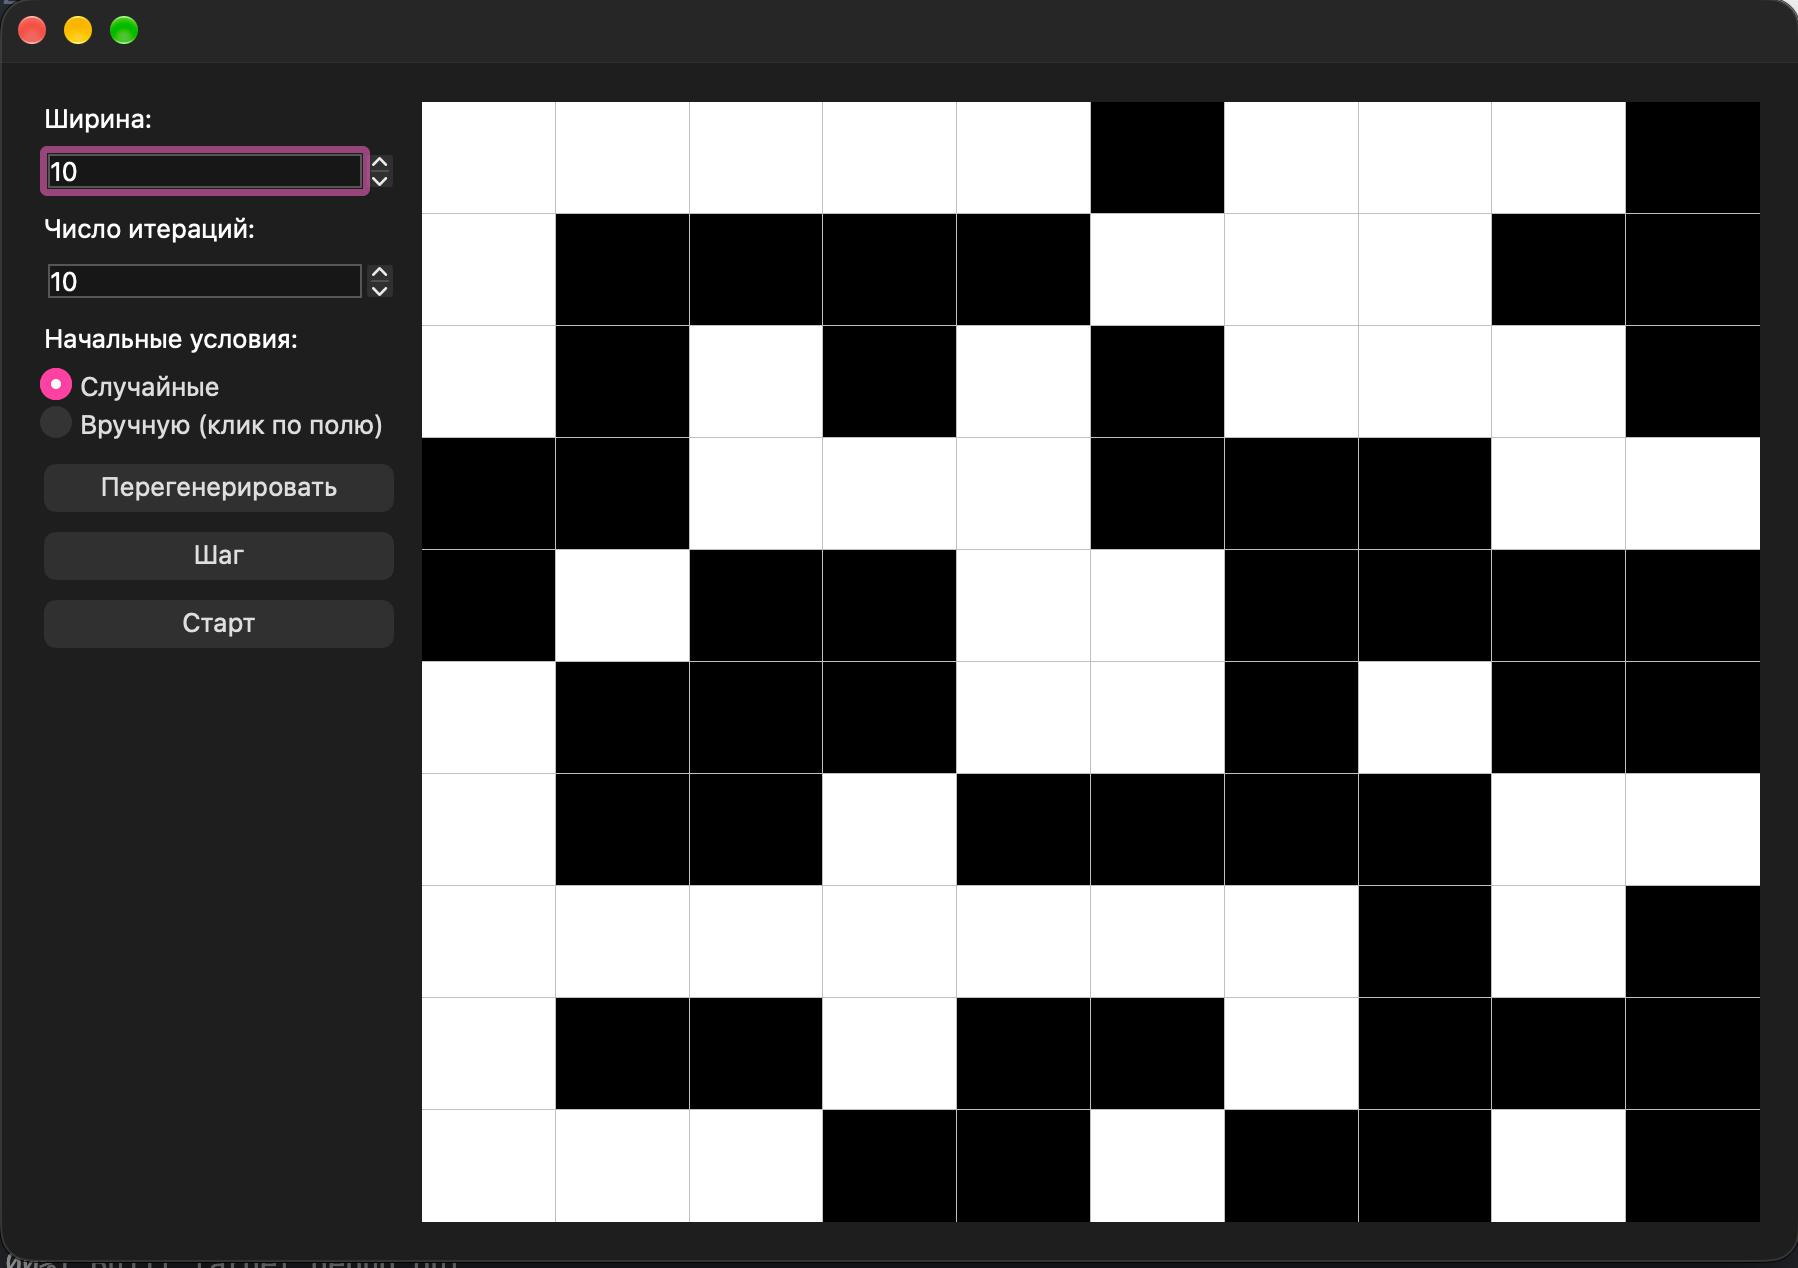
\includegraphics[width=\textwidth]{pic/random_t0.jpg}\\
  а) $t=0$ (начальное состояние)
 \end{minipage}
 \hfill
 \begin{minipage}{0.48\textwidth}
  \centering
  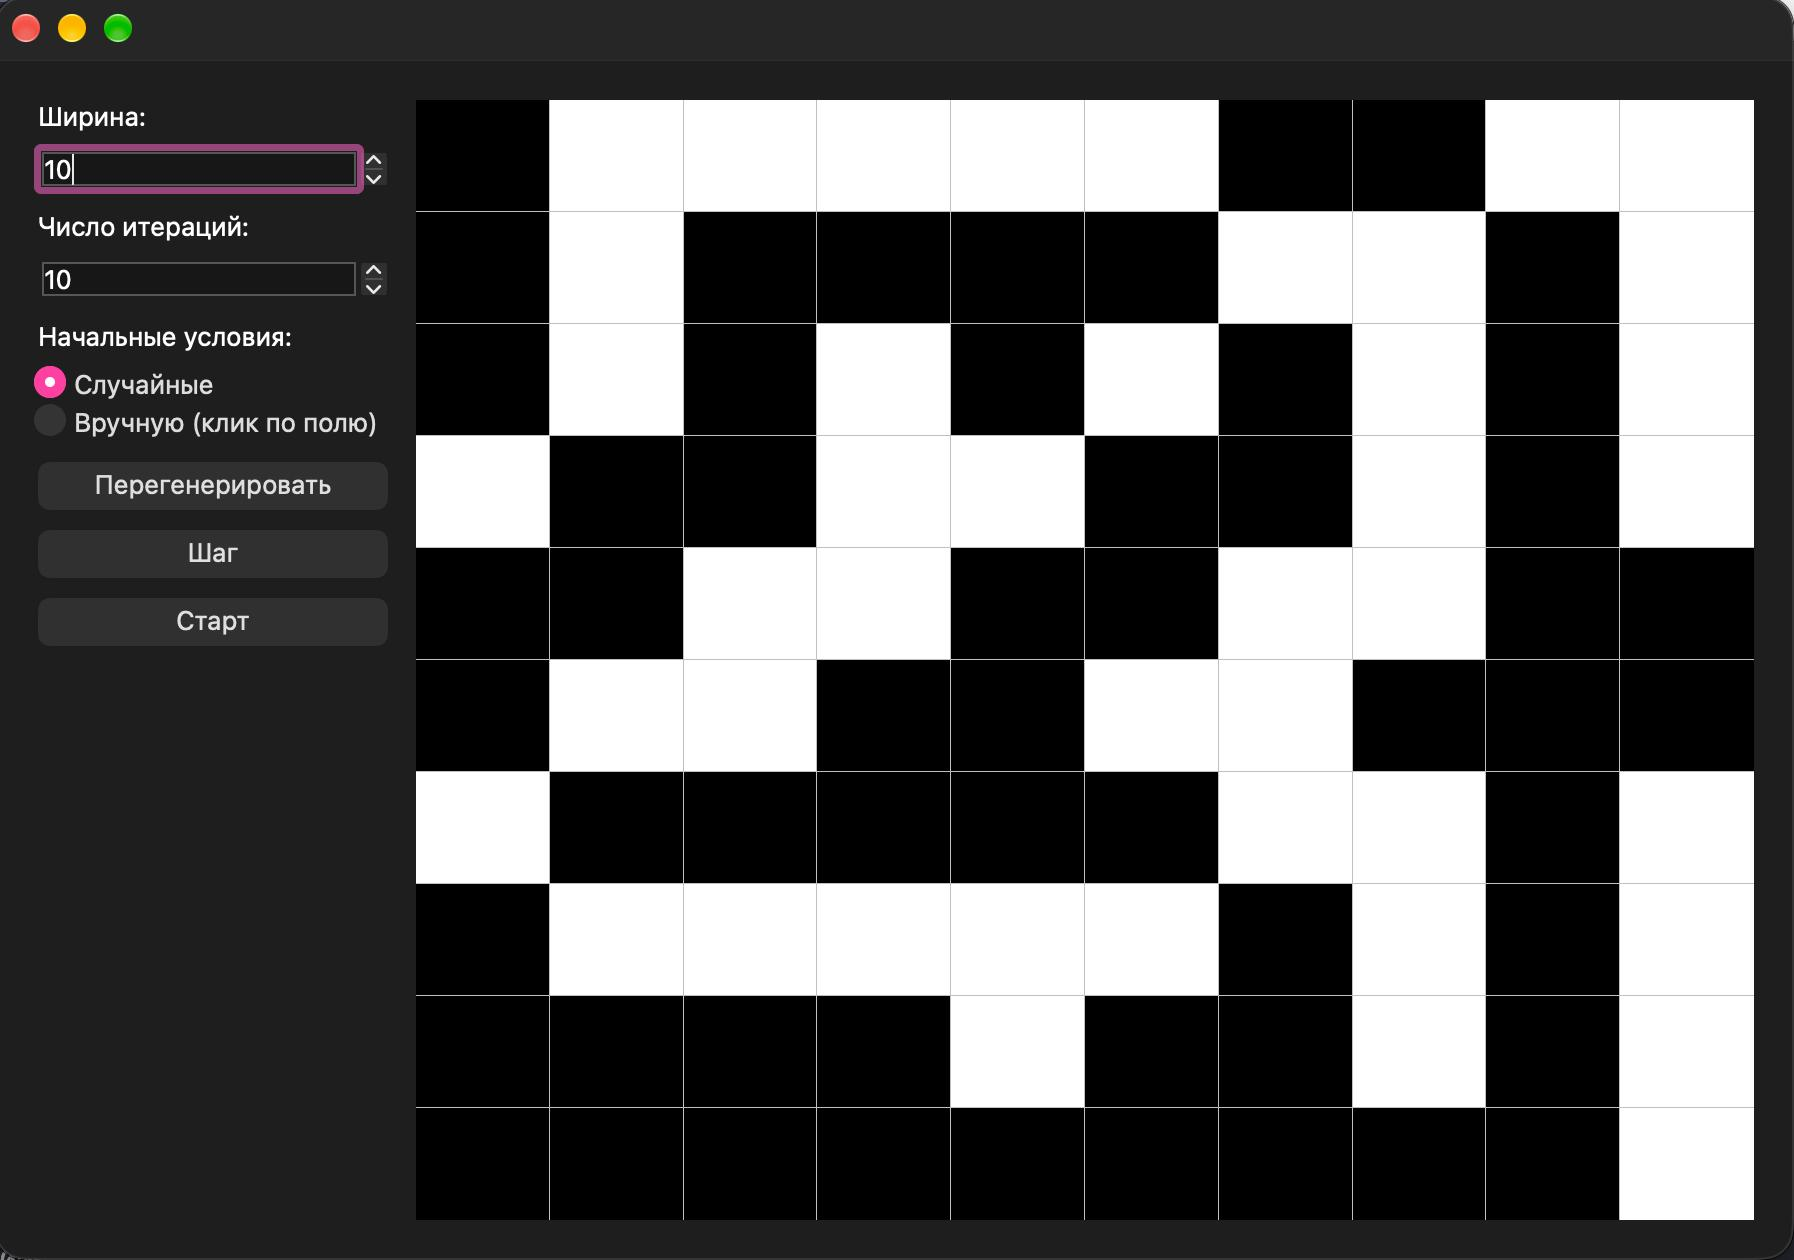
\includegraphics[width=\textwidth]{pic/random_t1.jpg}\\
  б) $t=1$
 \end{minipage}

 \vspace{0.5cm}

 \begin{minipage}{0.48\textwidth}
  \centering
  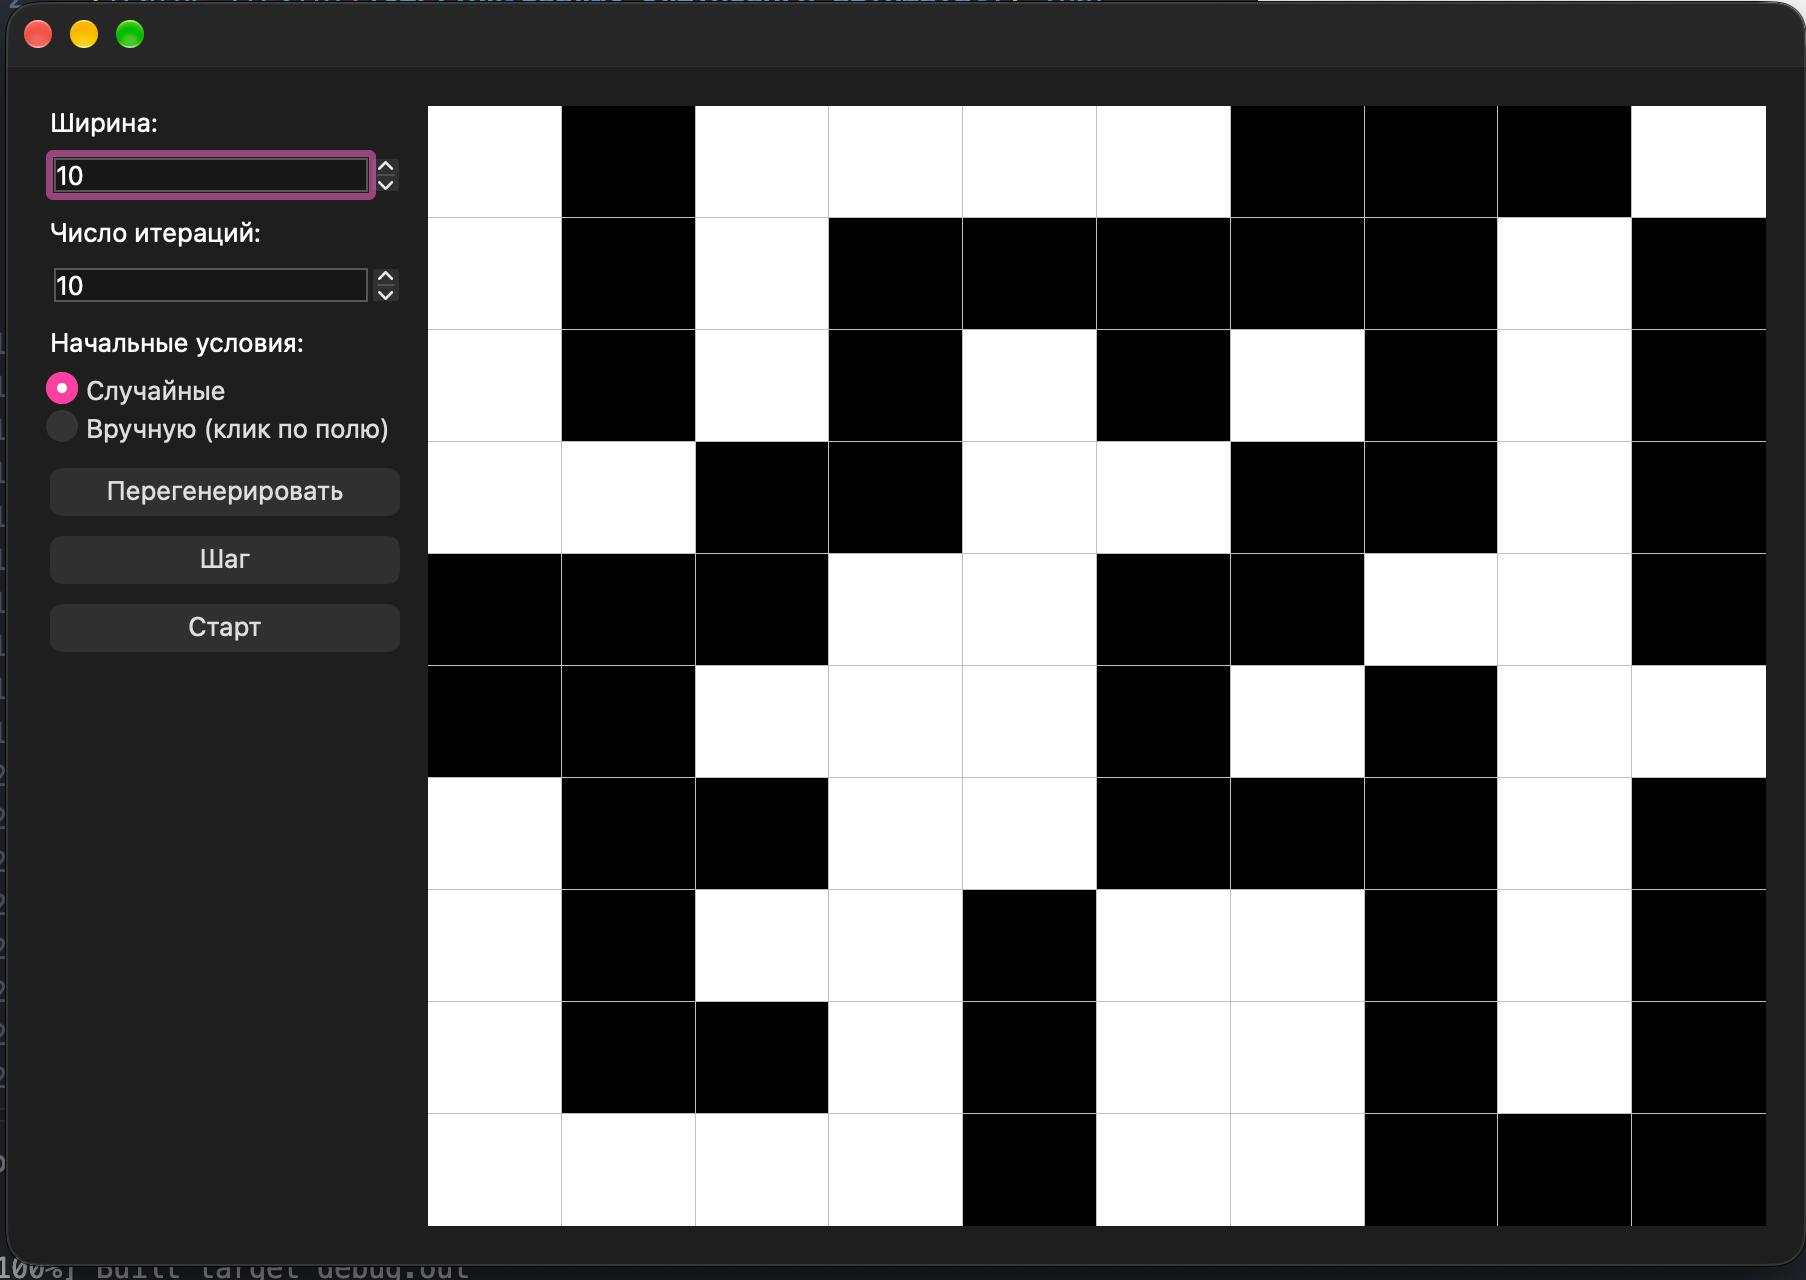
\includegraphics[width=\textwidth]{pic/random_t2.jpg}\\
  в) $t=2$
 \end{minipage}
 \hfill
 \begin{minipage}{0.48\textwidth}
  \centering
  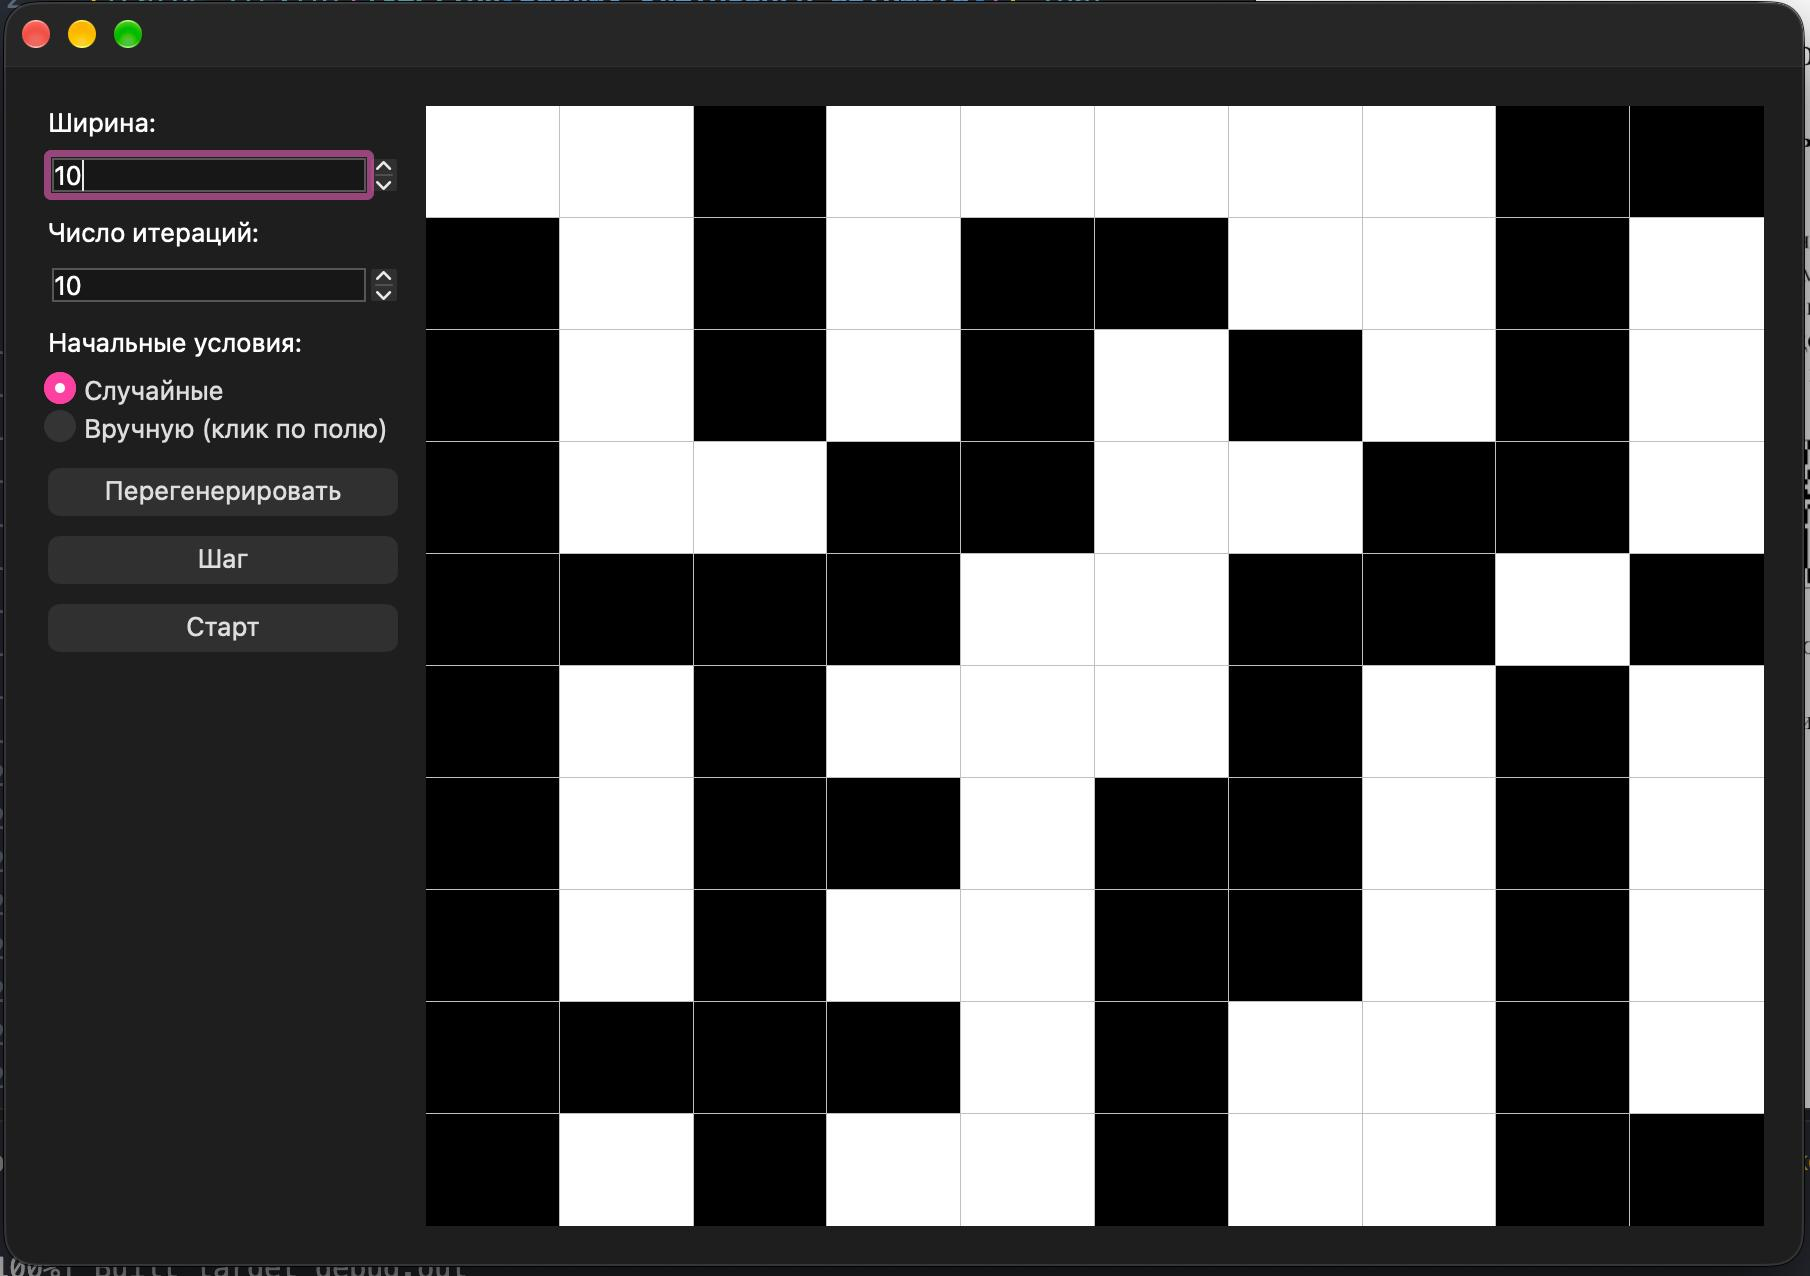
\includegraphics[width=\textwidth]{pic/random_t3.jpg}\\
  г) $t=3$
 \end{minipage}
 \caption{Первые три итерации на случайном поле $10\times 10$}
 \label{fig:random}
\end{figure}

\noindent{\Large \textbf{\subsection{Работа программы на ручных начальных условиях}}} \par

На рис.\ref{fig:manual} показаны начальное состояние, заданное вручную кликами по полю $10\times 10$, и первые пять итераций.

\begin{figure}[H]
 \centering
 \begin{minipage}{0.48\textwidth}
  \centering
  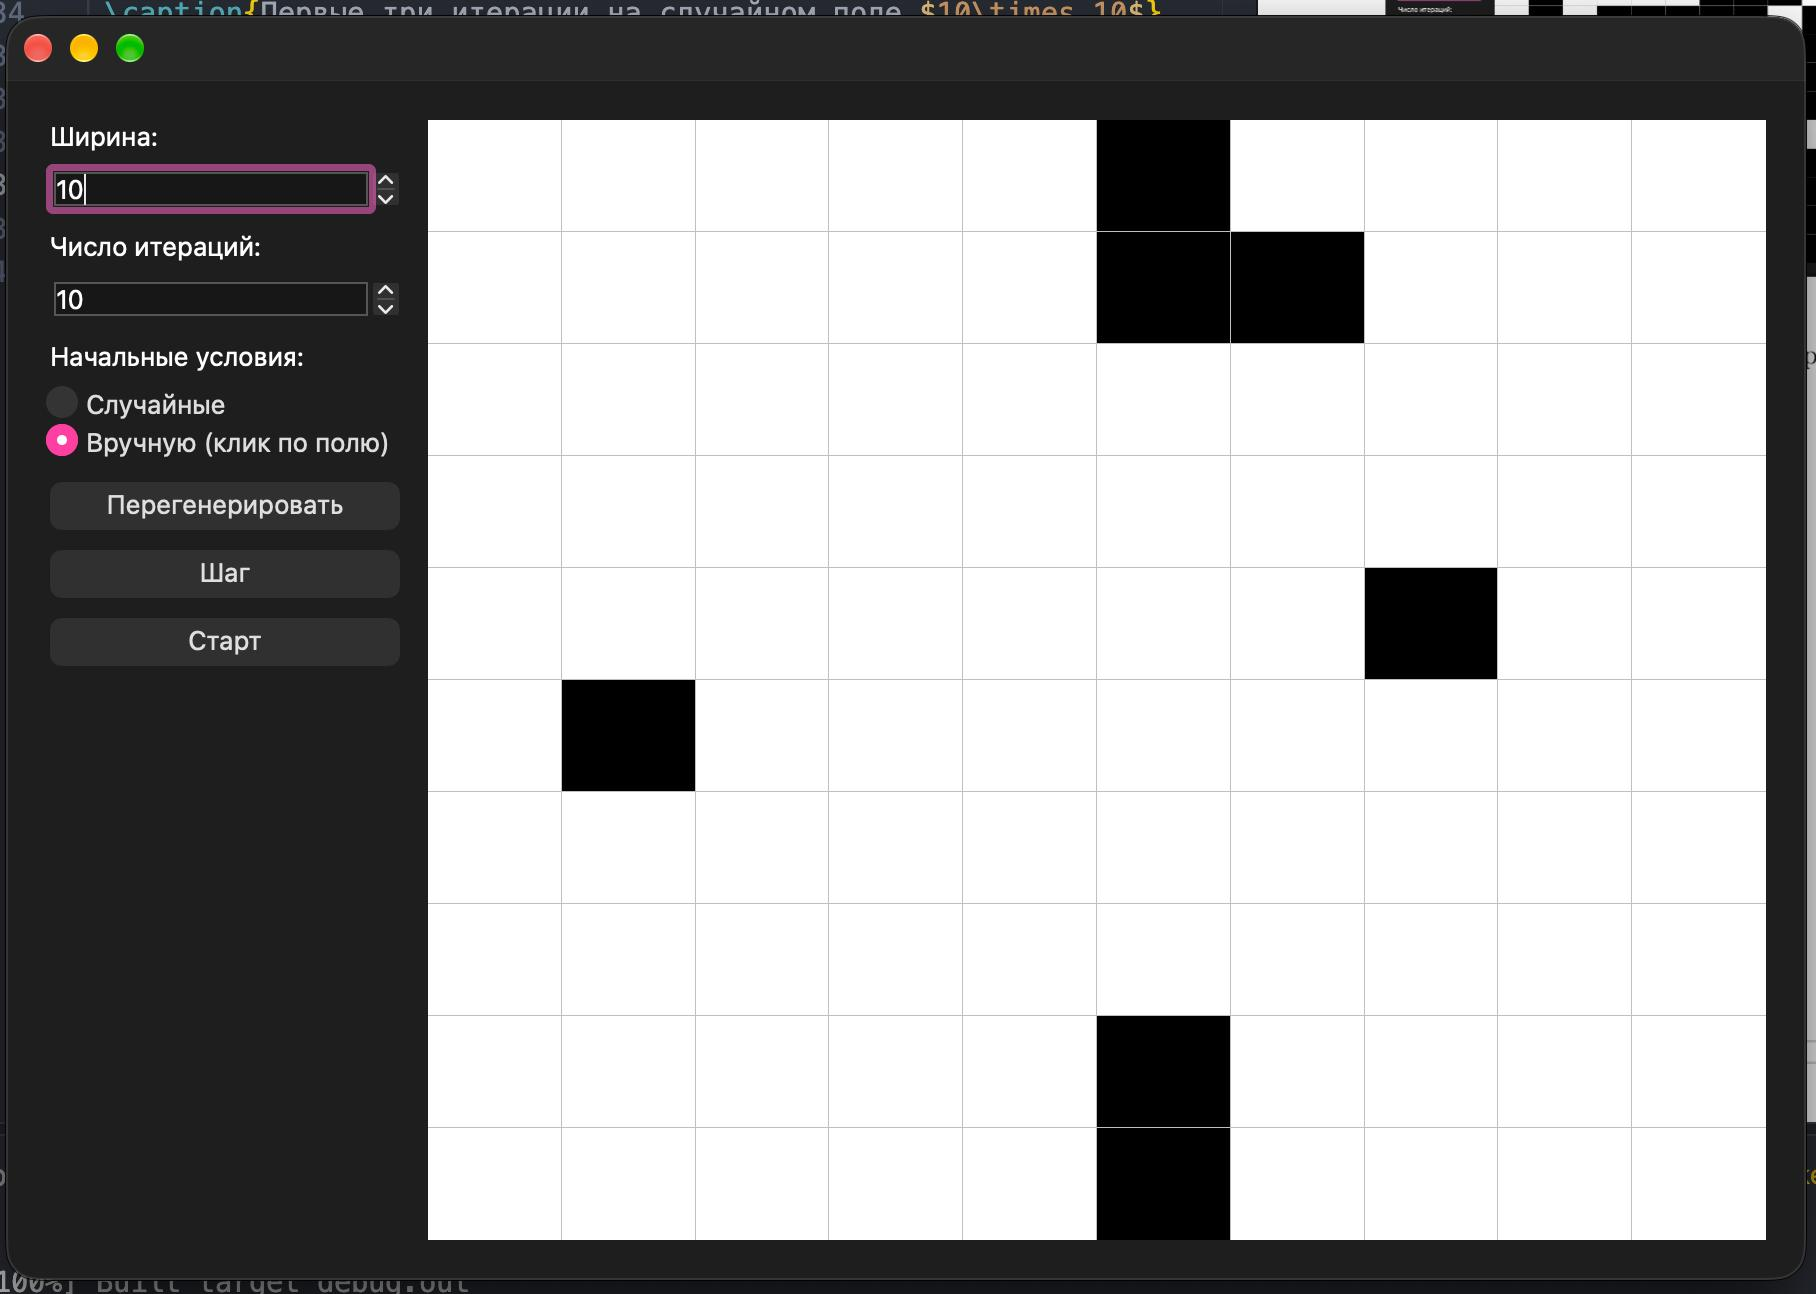
\includegraphics[width=\textwidth]{pic/manual_t0.jpg}\\
  а) $t=0$ (начальное состояние)
 \end{minipage}
 \hfill
 \begin{minipage}{0.48\textwidth}
  \centering
  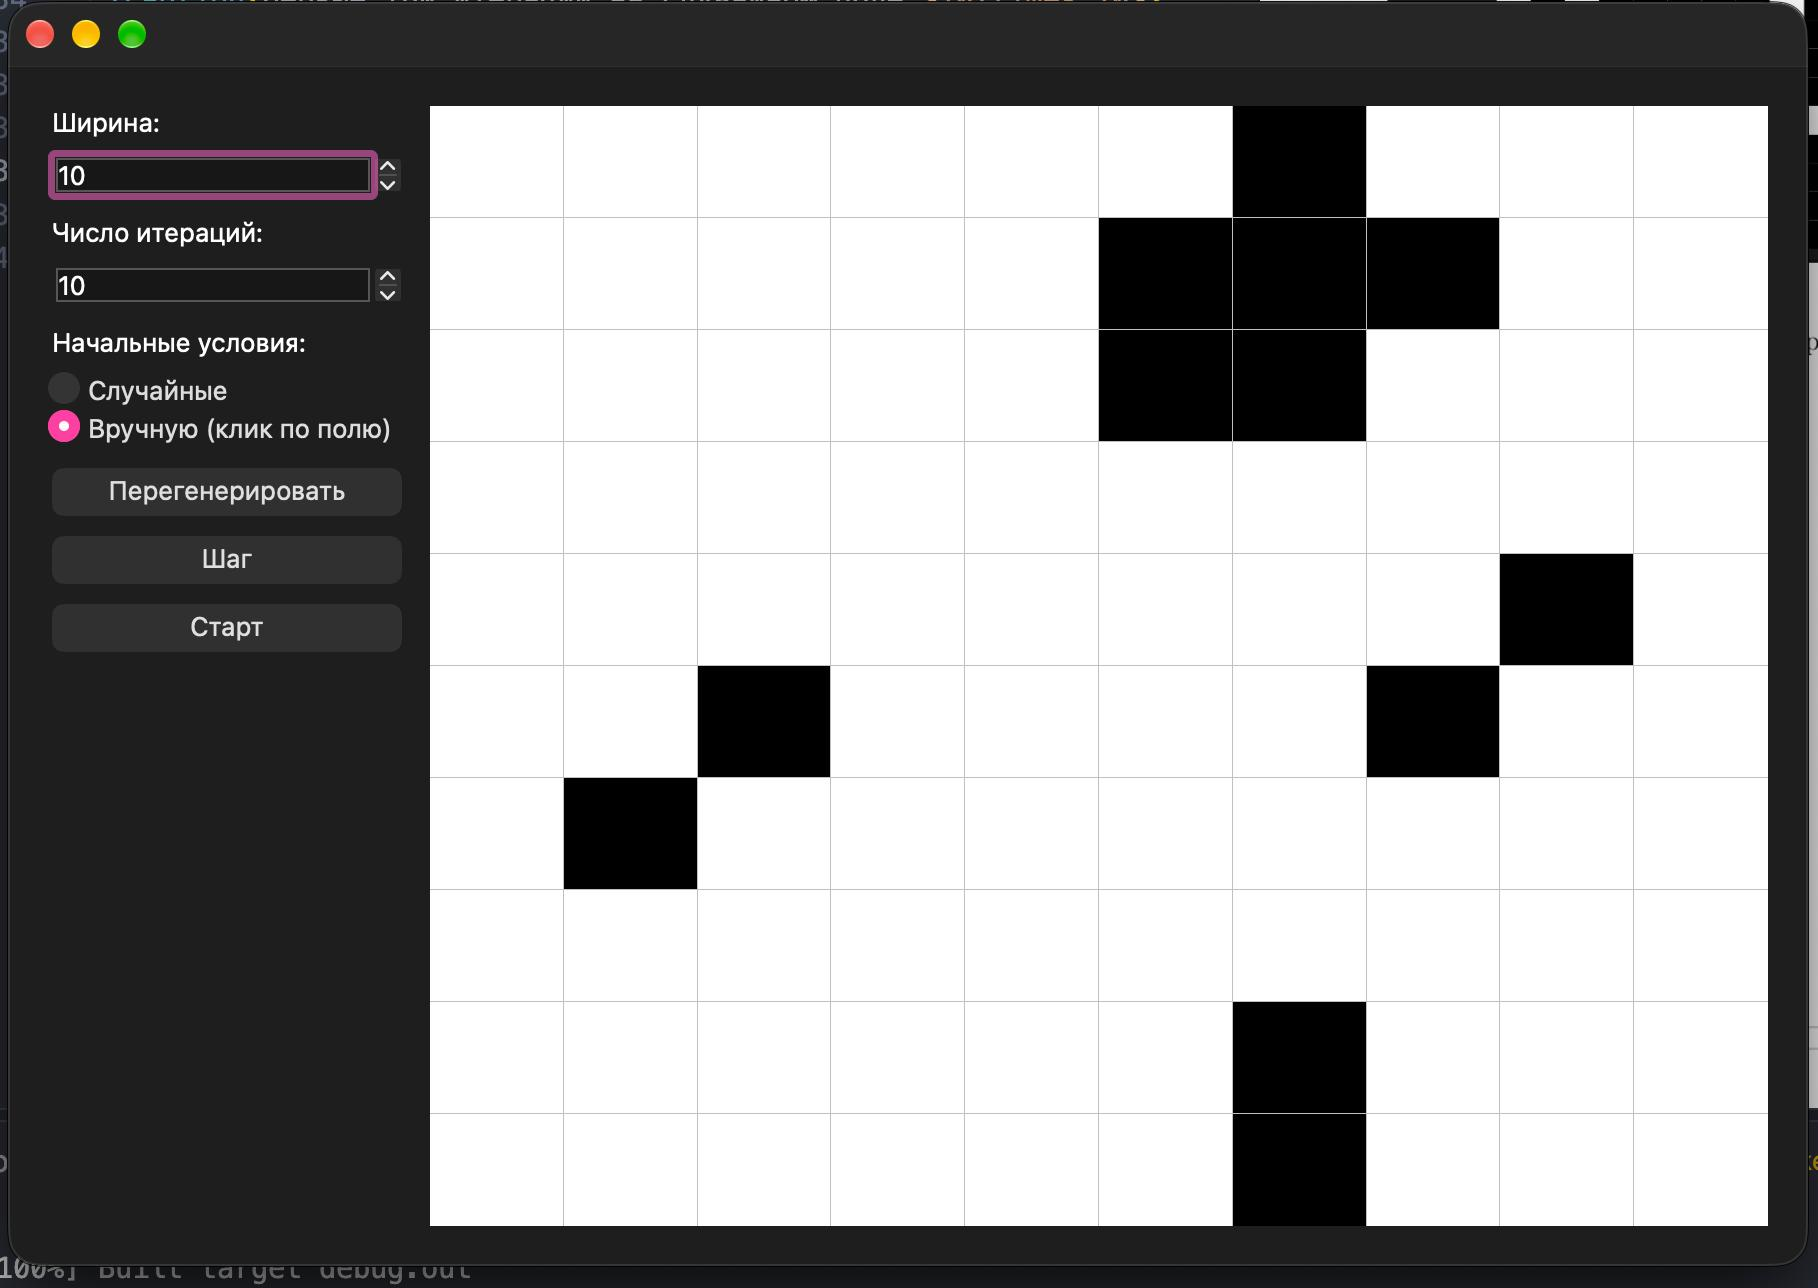
\includegraphics[width=\textwidth]{pic/manual_t1.jpg}\\
  б) $t=1$
 \end{minipage}

 \vspace{0.3cm}

 \begin{minipage}{0.48\textwidth}
  \centering
  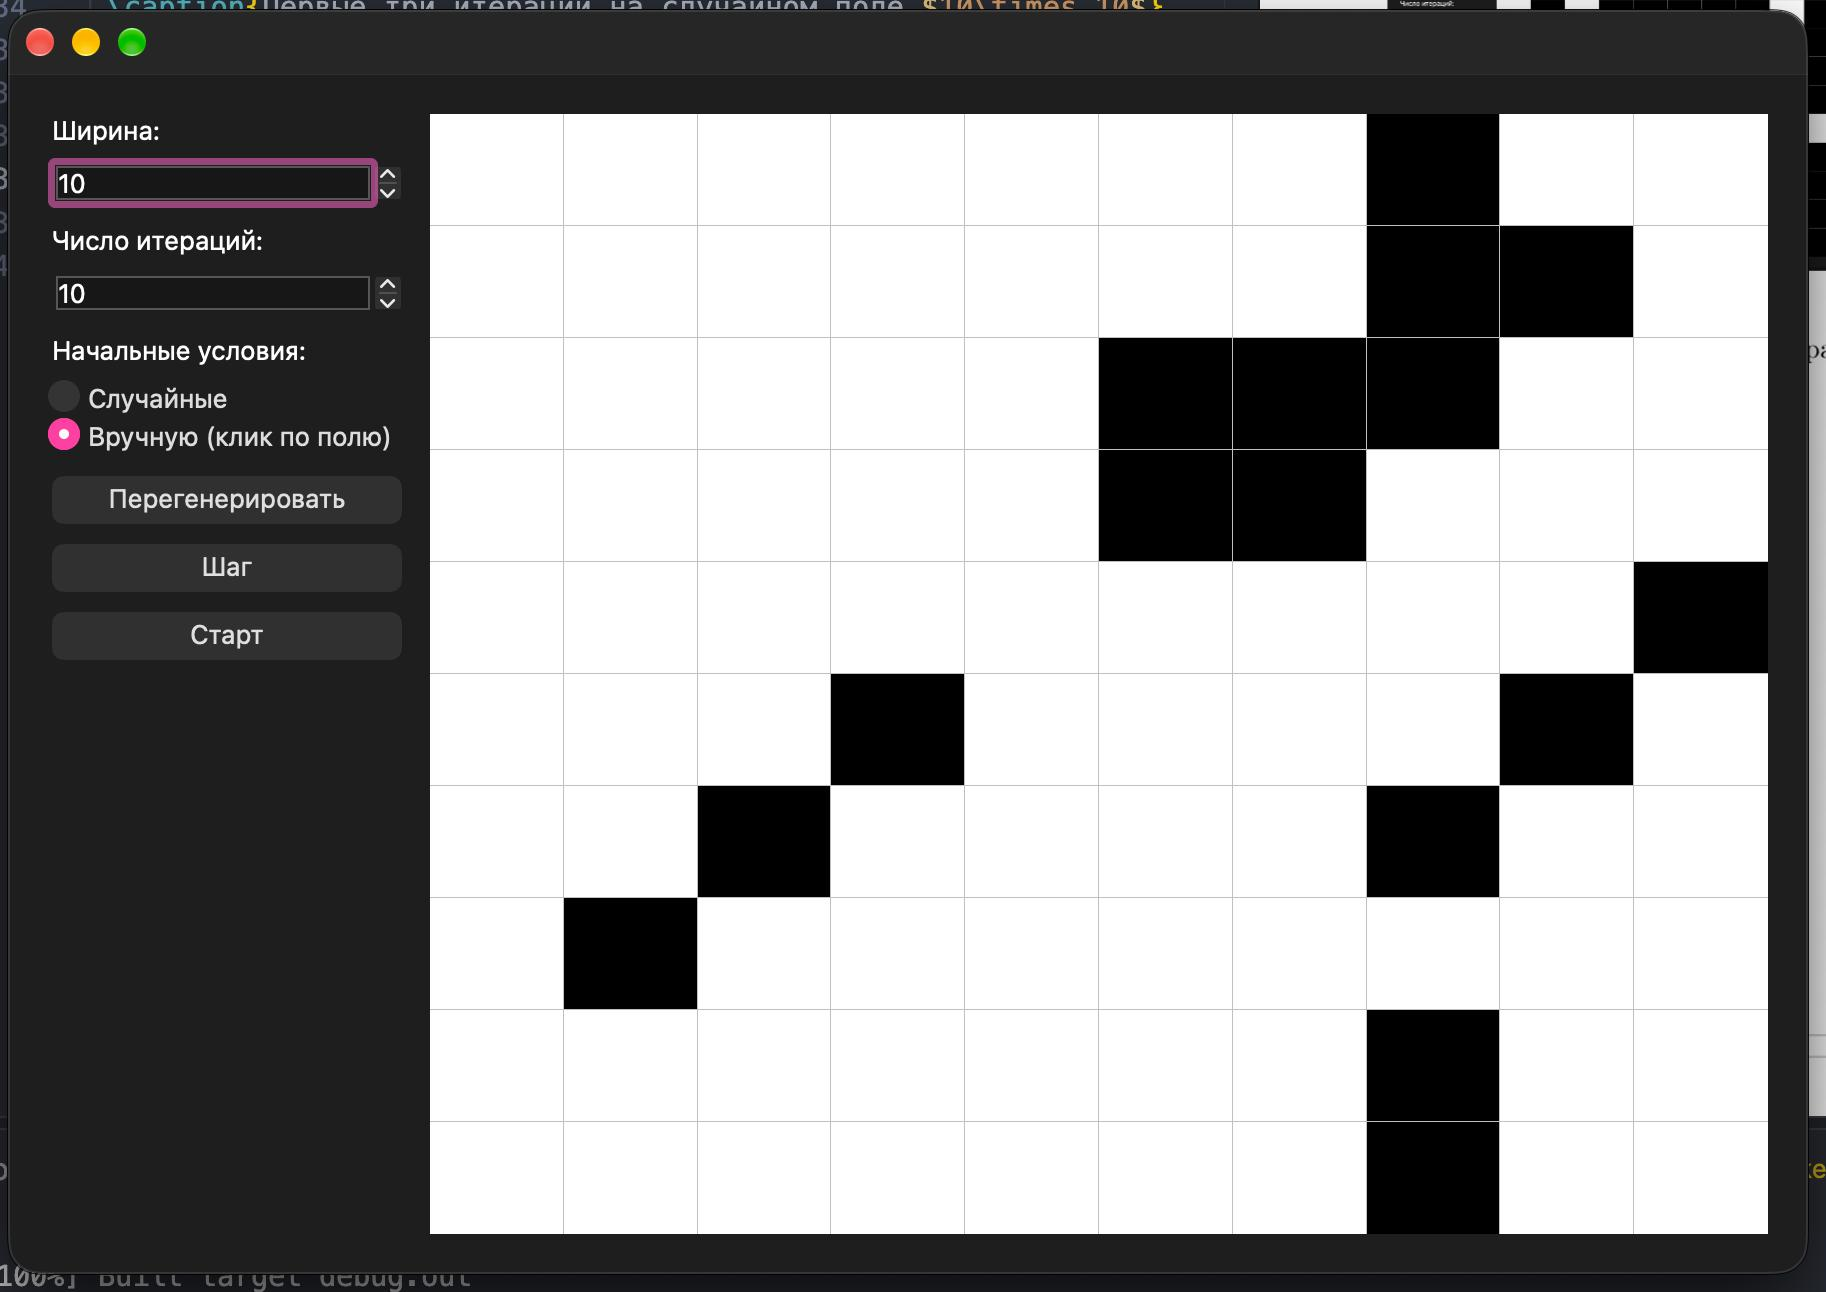
\includegraphics[width=\textwidth]{pic/manual_t2.jpg}\\
  в) $t=2$
 \end{minipage}
 \hfill
 \begin{minipage}{0.48\textwidth}
  \centering
  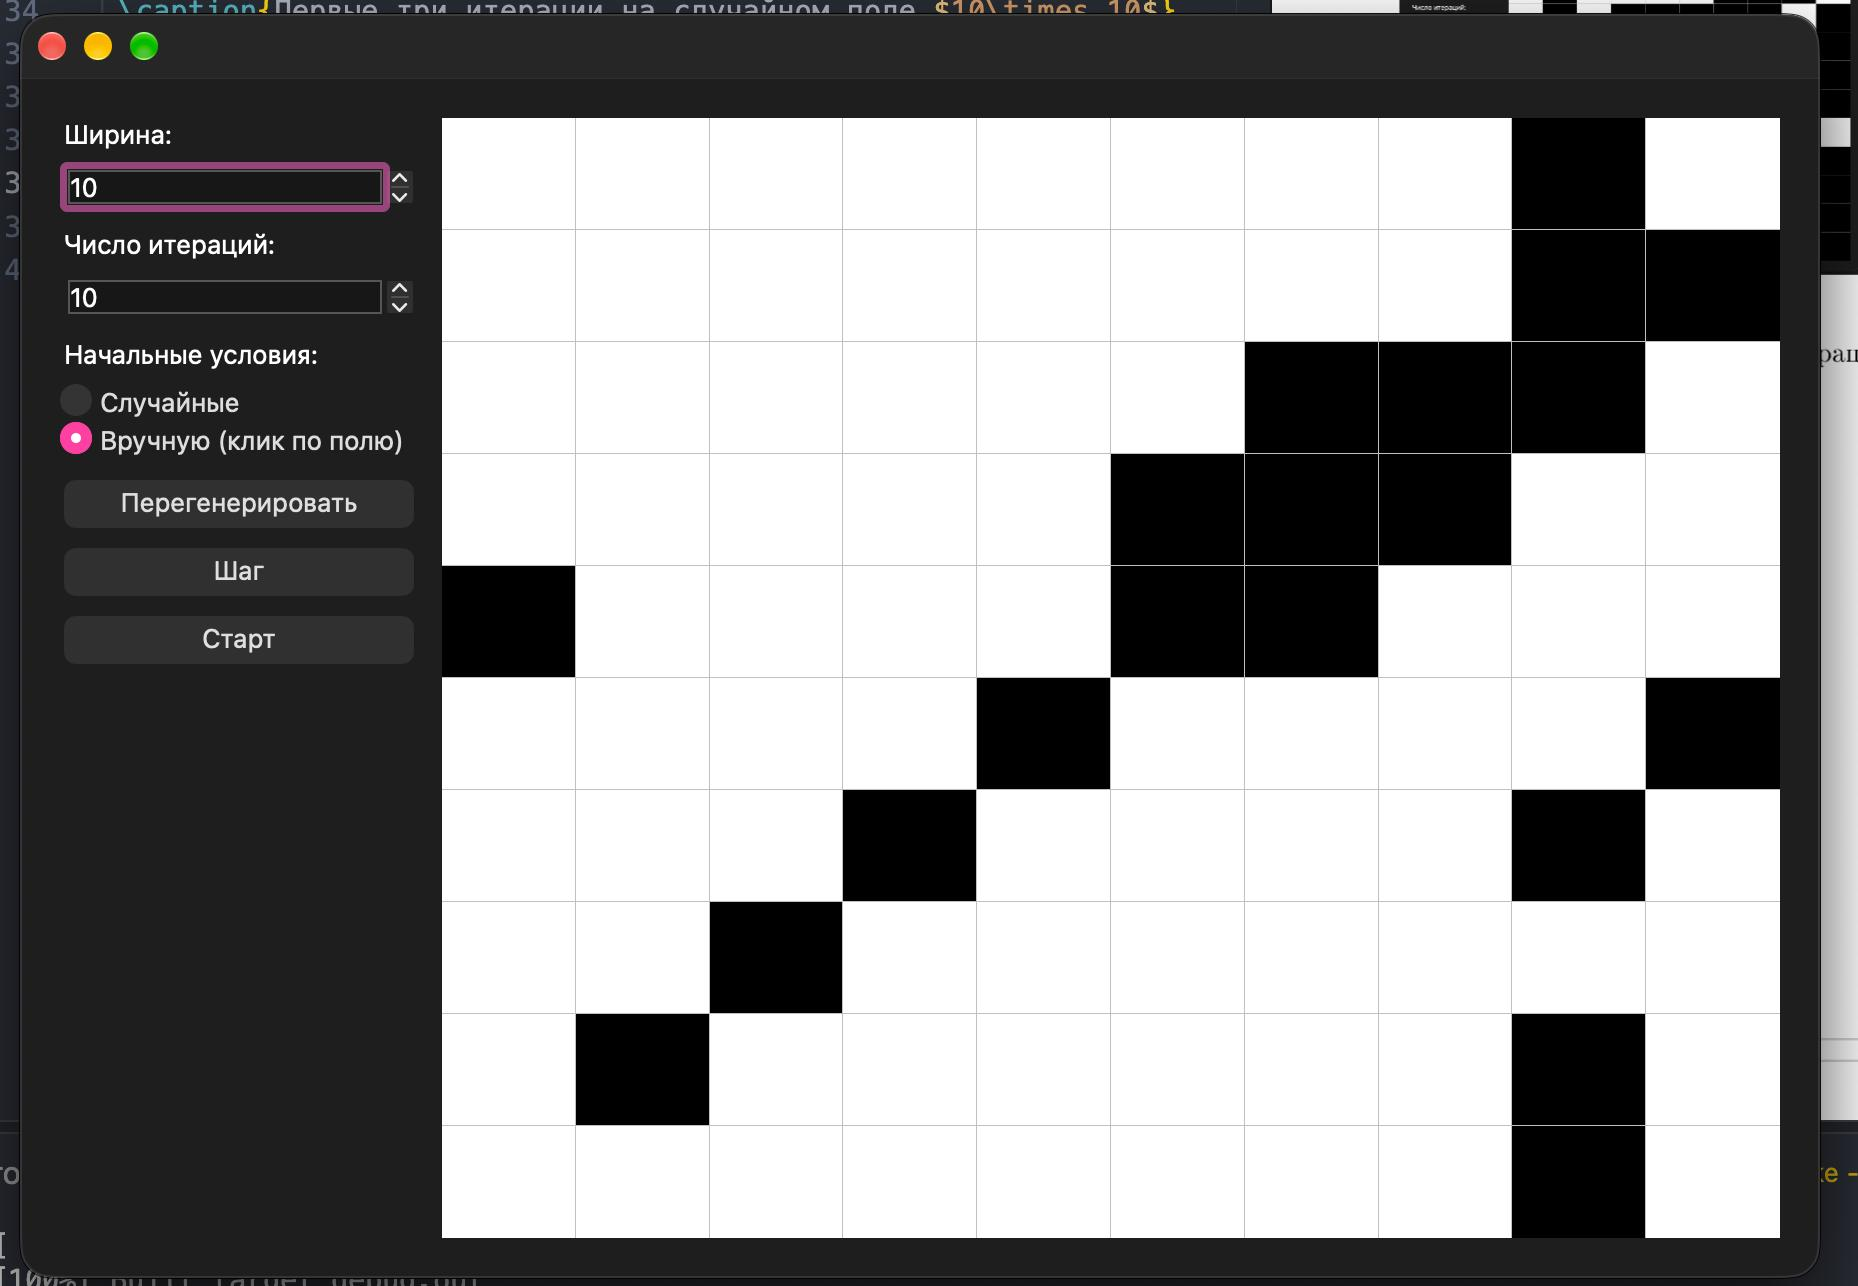
\includegraphics[width=\textwidth]{pic/manual_t3.jpg}\\
  г) $t=3$
 \end{minipage}

 \vspace{0.3cm}

 \begin{minipage}{0.48\textwidth}
  \centering
  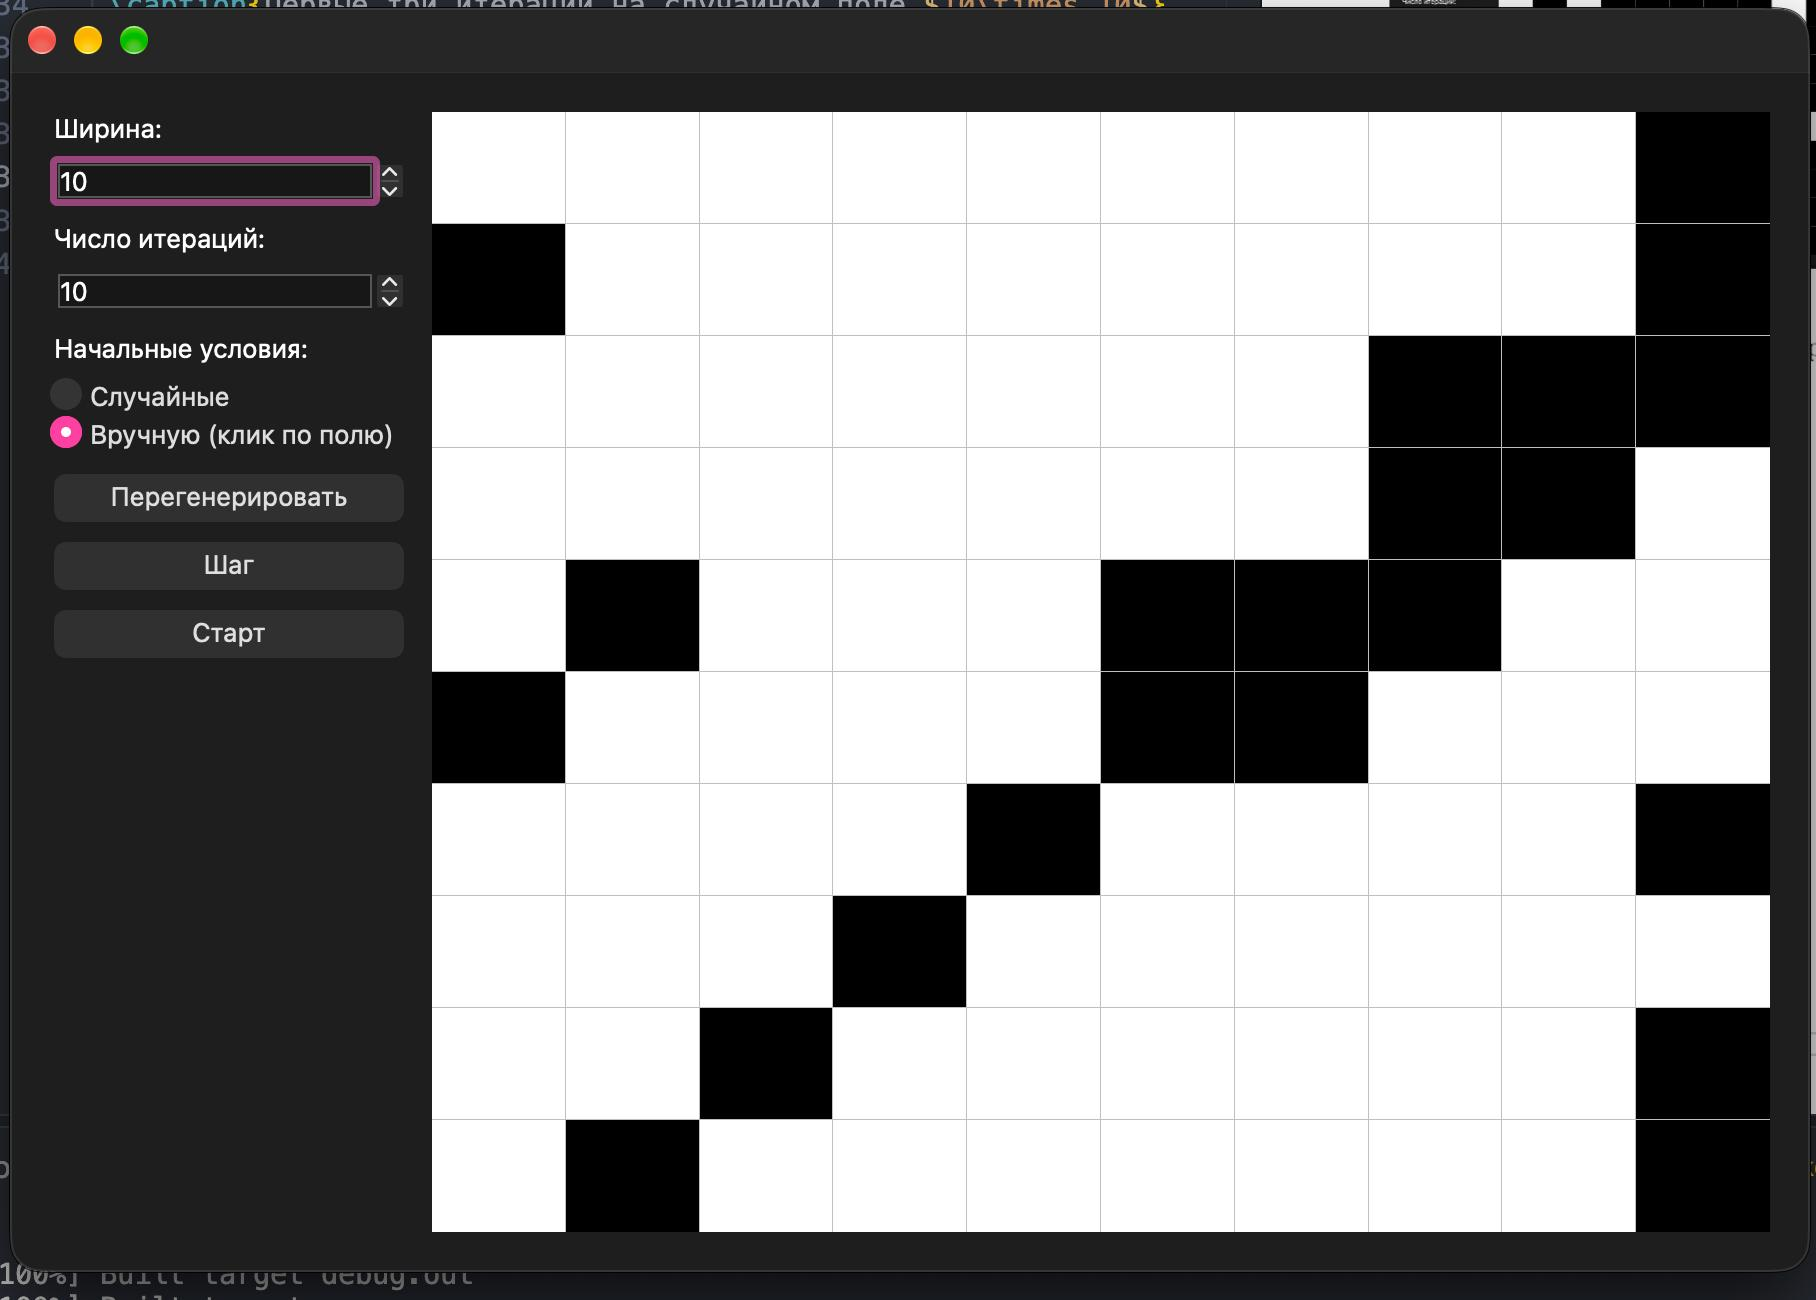
\includegraphics[width=\textwidth]{pic/manual_t4.jpg}\\
  д) $t=4$
 \end{minipage}
 \hfill
 \begin{minipage}{0.48\textwidth}
  \centering
  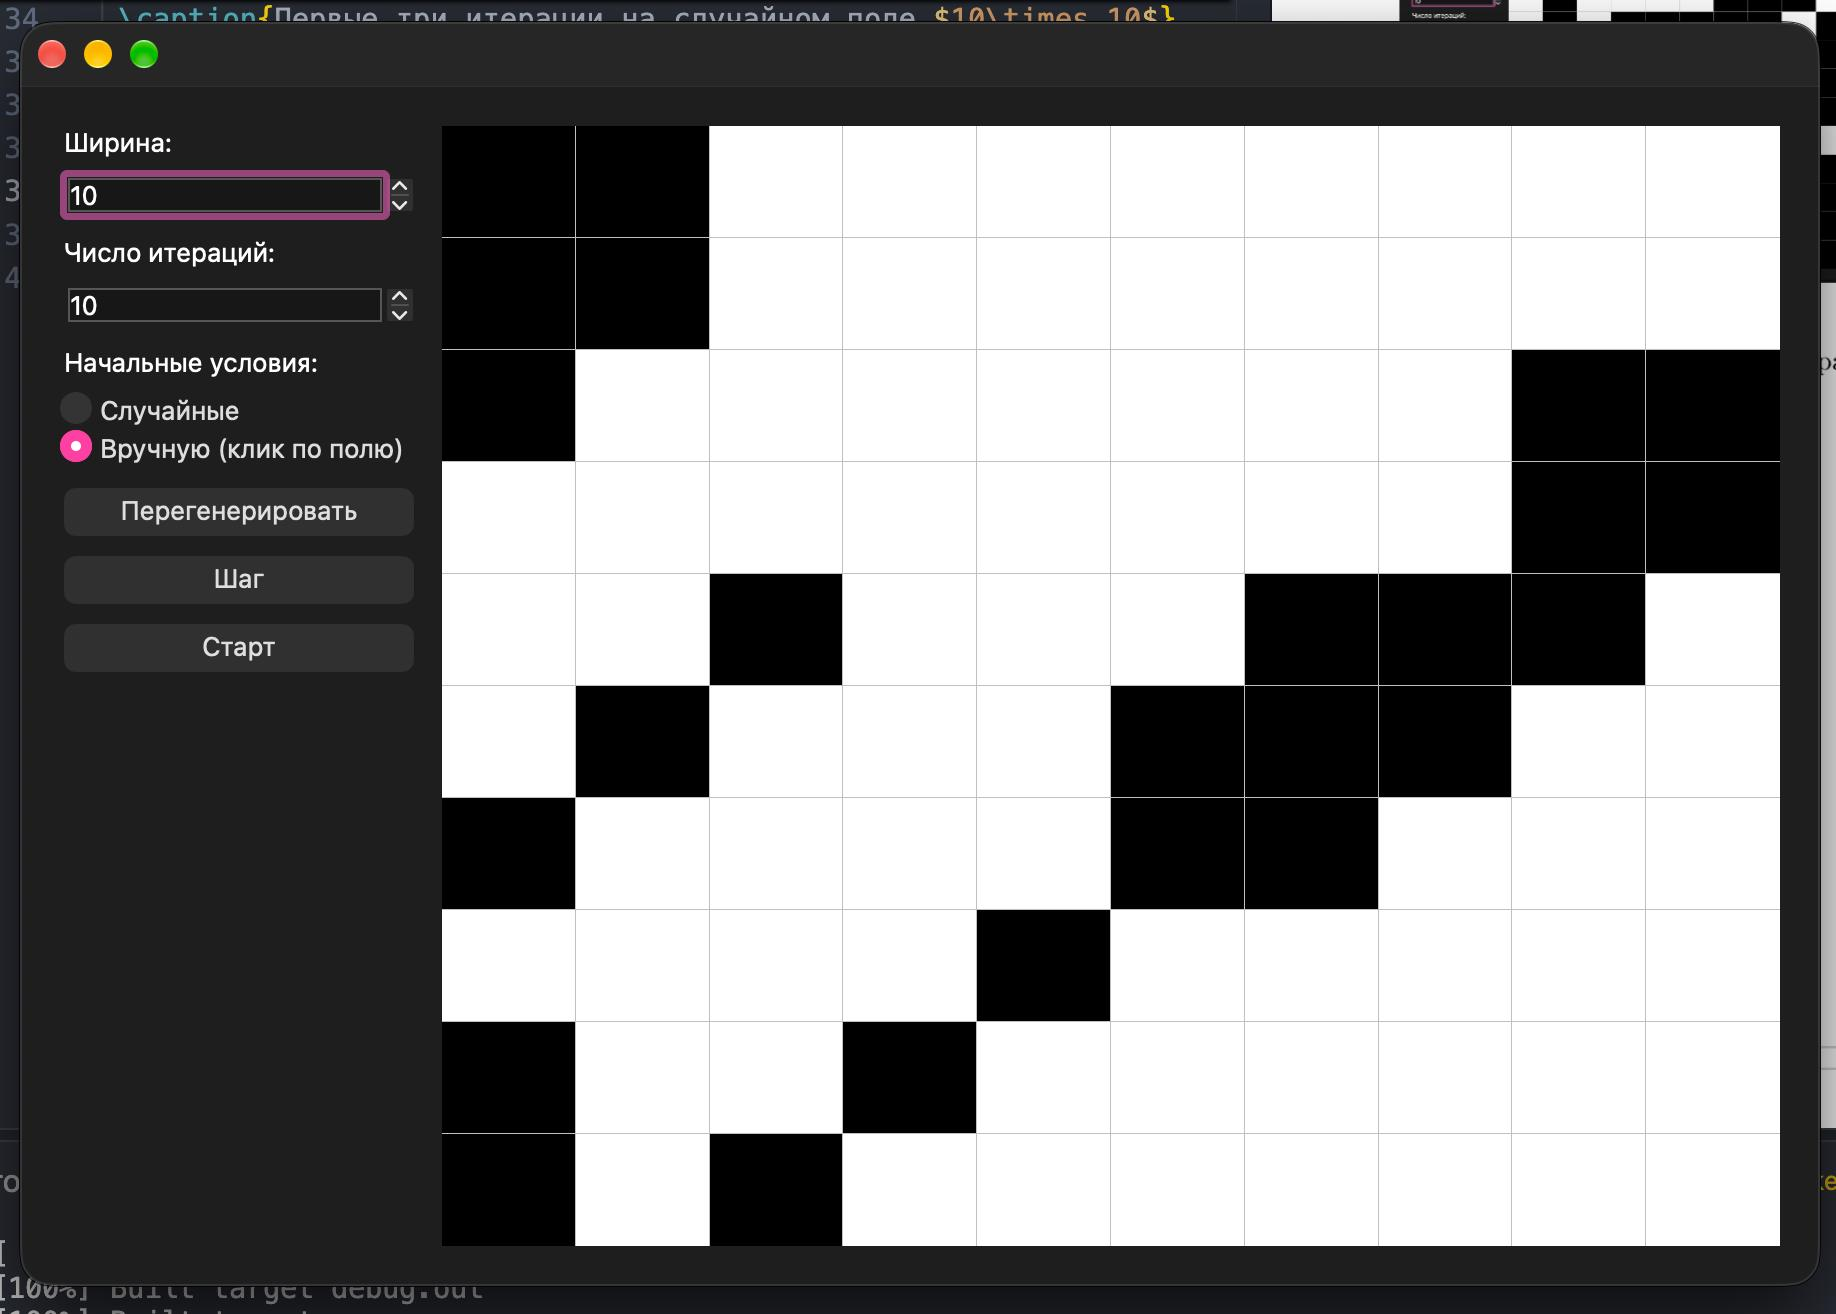
\includegraphics[width=\textwidth]{pic/manual_t5.jpg}\\
  е) $t=5$
 \end{minipage}
 \caption{Первые пять итераций при ручных начальных условиях, поле $10\times 10$}
 \label{fig:manual}
\end{figure}

\newpage


%Анализ клеточного автомата
\noindent
{\Large \textbf{\section{Анализ клеточного автомата}}} \par


\noindent{\Large \textbf{\subsection{Паттерны}}} \par

\noindent{\large \textbf{\subsubsection{Тривиальные начальные условия}}} \par

Для начала рассмотрим два тривиальных начальных условия, когда все клетки или одновременно живы, или мертвы.

Пустое поле неподвижно, так как $f(0,0,0,0,0)=0$, а полностью заполненное поле за один шаг становится пустым, так как $f(1,1,1,1,1)=0$.

При нетривиальных начальных условиях можно выделить два вида поведения: шахматные доски, которые на каждой итерации инвертируют клетки, и диагональные волны, которые дрейфуют по полю. Рассмотрим их отдельно.

{\large \textbf{\subsubsection{Шахматные доски}}} \par

Существуют две шахматные доски: с живой и с мертвой клеткой в левом верхнем углу. В любой из них все четыре соседа каждой клетки имеют цвет, противоположный цвету самой клетки, поэтому используются только две строки таблицы истинности:
\begin{itemize}[itemsep=-3pt]
 \item живая клетка с мертвыми соседями, $f(0,0,1,0,0)=0$ ($i=4$): клетка умирает
 \item мертвая клетка с живыми соседями, $f(1,1,0,1,1)=1$ ($i=27$): клетка оживает
\end{itemize}
Следовательно, на каждом шаге все клетки меняют цвет, $x_{t+1}=1-x_t$: одна доска заменяется другой, а через два шага возвращается в исходное состояние, то есть пара шахматных досок образует цикл периода $2$ шага (рис.\ref{fig:checker}).

Однако цвета чередуются в шахматном порядке только при чётной ширине поля из-за тороидальных граничных условий.
При нечетной ширине поля, после нескольких итераций поле прийдет к паттерну дрейфующих волн, описанному ниже.

\begin{figure}[H]
 \centering
 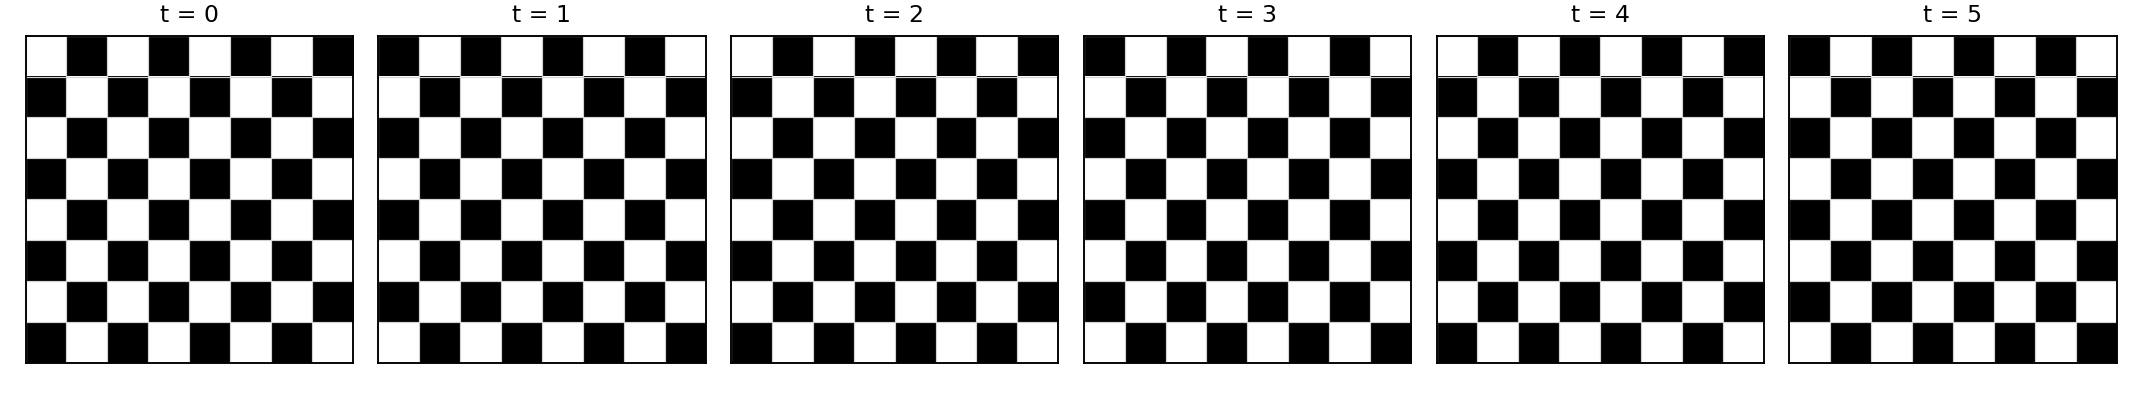
\includegraphics[width=0.55\textwidth]{pic/checkerboard.png}
 \caption{Шахматное поле $8\times 8$: цикл периода 2}
 \label{fig:checker}
\end{figure}

{\large \textbf{\subsubsection{Диагональные волны (дрейф вправо)}}} \par

В отличие от шахматных досок, здесь закрашенные клетки не стоят на месте, а смещаются вправо, закрашивая соседа по диагонали. Наиболее чистый пример даёт одиночная живая клетка (рис.\ref{fig:drift}).

Таким образом, на каждом шаге живая клетка исчезает, но передаёт жизнь соседу справа и соседу снизу. Эти две новые клетки лежат на одной диагонали, поэтому из одной клетки возникает диагональный отрезок. 

Волна на торе ширины $n$ замыкается при $t=n-1$, диагональ при этом состоит из $n$ клеток.

\begin{figure}[H]
 \centering
 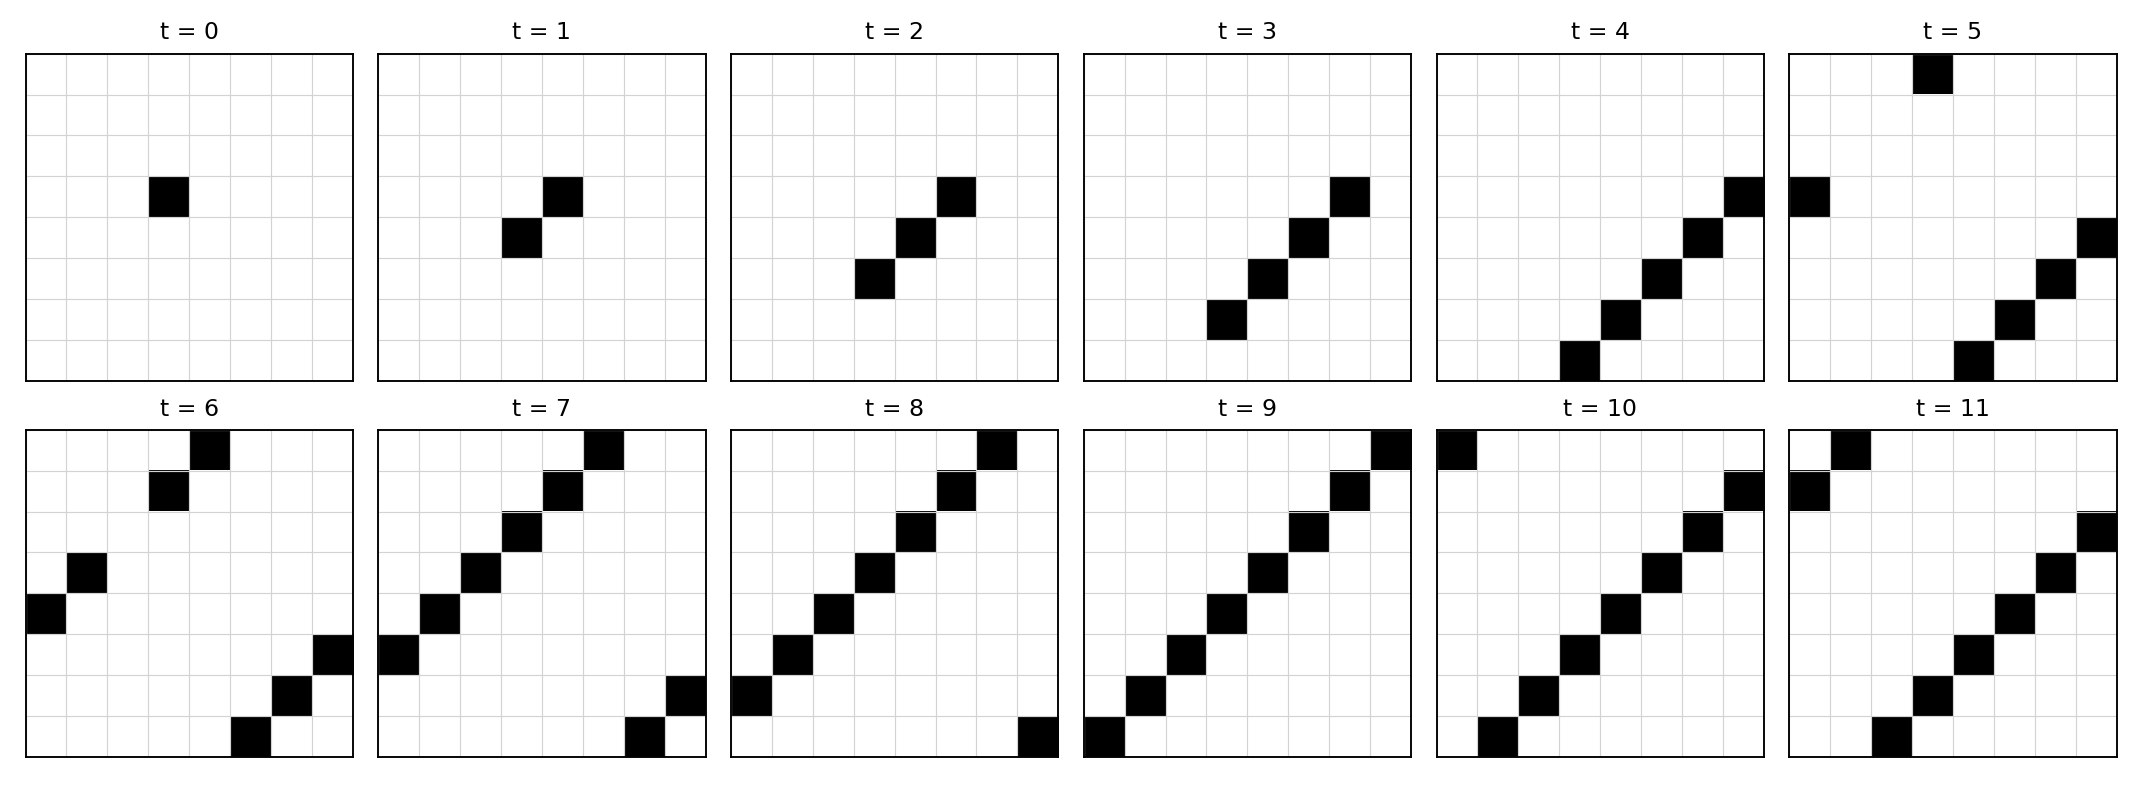
\includegraphics[width=\textwidth]{pic/drift.png}
 \caption{Диагональная волна на торе $10\times 10$}
 \label{fig:drift}
\end{figure}


% \noindent{\Large \textbf{\subsection{Плотность}}} \par

% Доля живых клеток быстро выходит на уровень около $0{,}5$ и далее лишь слабо колеблется (рис.\ref{fig:density}). При случайном старте с плотностью $1/2$ в аттракторе она лежит в пределах $0{,}46$-$0{,}54$. Если начальная плотность сильно отличается от $1/2$, система все равно «стягивается» к середине, но не полностью: плотность при $t=200$ составляет около $0{,}39$ при старте $0{,}05$ и около $0{,}34$ при старте $0{,}95$ (рис.\ref{fig:density_init}).

% \begin{figure}[H]
%  \centering
%  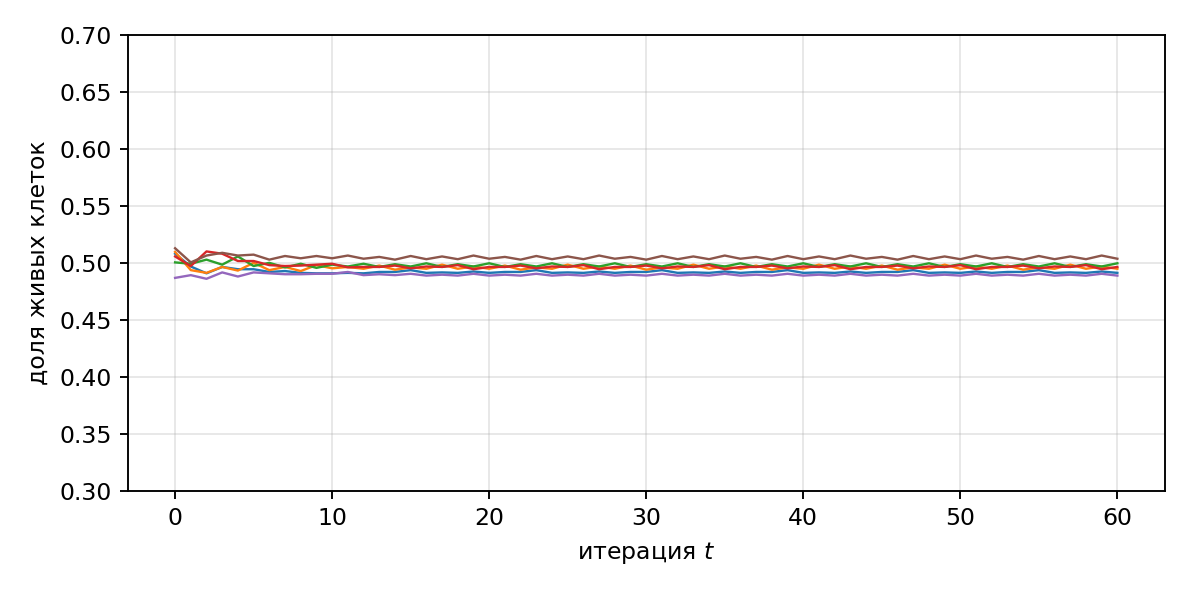
\includegraphics[width=0.75\textwidth]{pic/density.png}
%  \caption{Доля живых клеток при шести случайных стартах, поле $50\times 50$}
%  \label{fig:density}
% \end{figure}

% \begin{figure}[H]
%  \centering
%  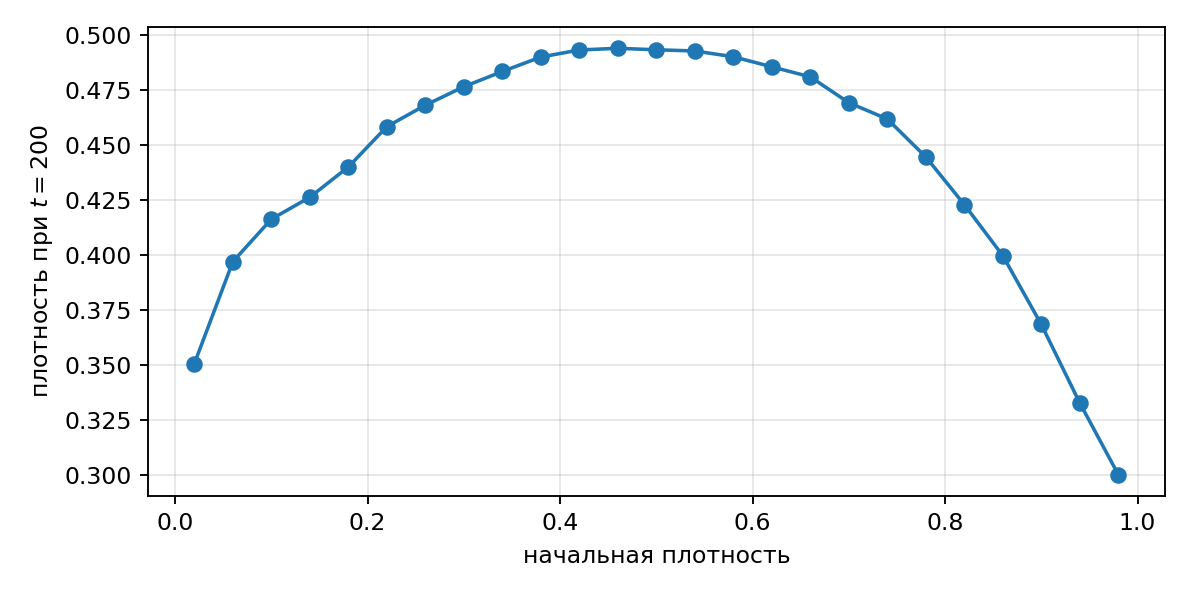
\includegraphics[width=0.75\textwidth]{pic/density_vs_init.png}
%  \caption{Плотность при $t=200$ в зависимости от начальной плотности (поле $40\times 40$, среднее по 15 запускам)}
%  \label{fig:density_init}
% \end{figure}

% Наблюдения:
% \begin{enumerate}[itemsep=-3pt]
%  \item Автомат всегда сходится не к неподвижной точке, а к \textbf{циклу}; ни одна случайная конфигурация не привела к вырождению в пустое или заполненное поле.
%  \item Предпериод короток и растет очень медленно (порядка $10$-$13$ шагов при росте $n$ с $20$ до $50$), т.е. локальный порядок формируется быстро, независимо от размеров поля.
%  \item \textbf{Период в 100\,\% наблюдавшихся запусков кратен ширине поля $n$} (например, $20$, $40$ для $n=20$; $60$, $120$ для $n=30$; $100$, $200$ для $n=50$). Это означает, что устойчивые структуры не стоят на месте, а перемещаются по полю с постоянной скоростью (порядка одной клетки за шаг) и возвращаются в исходное положение, обойдя тор. Тороидальные границы здесь существенны: период определяется длиной «обхода» тора.
% \end{enumerate}

\noindent{\Large \textbf{\subsection{Классификация по Вольфраму}}} \par

По наблюдаемому поведению автомат следует отнести к классу II, так как из случайного начального состояния он за короткое время переходит к набору периодических структур. Однако данная классификация носит оценочный характер, так как строгих критериев классификации Вольфрама не существует.

\newpage


%Заключение
\noindent
{\Large \textbf{\section*{Заключение}}} \par
\addcontentsline{toc}{section}{Заключение} \par

В ходе выполнения лабораторной работы реализован двумерный клеточный автомат с окрестностью фон Неймана и тороидальными границами по варианту $N=50045688$. 

Реализовано:
\begin{enumerate}[itemsep=-3pt]
 \item Правило перехода в соответствии с номером варианта (таблица истинности булевой функции 5 переменных)
 \item Поле с тороидальными граничными условиями
 \item Возможность изменения начальных условий: ширины поля, числа итераций, типа генерации, режима работы (автоматический или пошаговый)
\end{enumerate}

\textbf{Достоинства реализованного решения:}
\begin{enumerate}[itemsep=-3pt]
 \item Правило перехода строится из исходного числа автоматически, поэтому для другого варианта достаточно изменить одну константу.
 \item Пользователю предоставлено два режима работы программы: с заданным числом итераций и пошаговый.
 \item Таблица истинности строится один раз в конструкторе и хранится в ассоциативном массиве из 32 элементов, поэтому при вычислении шага для клетки нужен лишь поиск по ключу (не более $\log_2 32 = 5$ сравнений), а не вычисление значения булевой функции.
\end{enumerate}

\textbf{Недостатки и возможности для улучшения:}
\begin{enumerate}[itemsep=-3pt]
 \item Номер текущей итерации хранится в программе, но не отображается в интерфейсе, также нет вывода статистики (например, доли живых клеток). Для этого можно реализовать отдельный виджет со статистикой.
 \item Кнопка «Перегенерировать» не останавливает таймер. Если нажать её во время автоматического режима, оставшиеся итерации продолжат выполняться уже на новом поле. Решение - останавливать таймер и сбрасывать счетчик оставшихся шагов в \texttt{on\_init}
\end{enumerate}

\textbf{Масштабируемость решения:}
\begin{enumerate}[itemsep=-3pt]
    \item Добавить возможность сохранять и загружать файлы с состоянием поля.
    \item Добавить поддержку правил, основанных не только на окрестности фон Неймана, но и на окрестности Мура.
    \item Добавить возможность делать шаг не только вперед ($t+1$), но и назад ($t-1$).
\end{enumerate}

\newpage


%Список литературы
\addcontentsline{toc}{section}{Список литературы} \par

\begin{thebibliography}{}
    \bibitem{temaspbstu} Лекции ВШТИИ по теории алгоритмов [Электронный ресурс]. URL: \href{https://tema.spbstu.ru/algorithm/}{https://tema.spbstu.ru/algorithm/} (дата обращения: 04.10.2026)

    \bibitem{itmo} Модели клеточных автоматов - Викиконспекты ИТМО [Электронный ресурс]. URL: \href{https://neerc.ifmo.ru/wiki/index.php?title=Модели_клеточных_автоматов}{https://neerc.ifmo.ru/wiki} (дата обращения: 04.10.2026).

    \bibitem{wolfram} Wolfram, Stephen, A New Kind of Science. Wolfram Media, Inc., May 14, 2002.

\end{thebibliography}
\newpage


%Приложение
%\input{src/Attachment}

\end{document}